% ----------------------------------------------------------------------
%                   Latex File for Joseph Roche's PhD (2012)
% ----------------------------------------------------------------------

%Latext thesis template from Harish Bhanderi's PhD/MPhil template, then Uni Cambridge
% http://www-h.eng.cam.ac.uk/help/tpl/textprocessing/ThesisStyle/

%: Style file for Latex
% Most style definitions are in the external file PhDthesisPSnPDF.
% In this template package, it can be found in ./Latex/Classes/
\documentclass[a4paper,oneside,12pt,usenatbib]{Latex/Classes/PhDthesisPSnPDF}
\setcitestyle{numbers}

%Change "oneside" to "twoside" for final submission-grade thesis after viva/corrections

\usepackage{lineno}
\usepackage{amsbsy}
\usepackage{amsmath}
\usepackage{xspace}
\usepackage{wtmmPkg}
%\usepackage{natbib}
\usepackage{multirow}
\usepackage{paralist}
%\usepackage{titlesec}
\usepackage{lscape}
\usepackage{quotchap}
\usepackage{epstopdf}
\usepackage{fancyhdr}
\usepackage{url}
\usepackage{hyperref}
\usepackage[capitalise]{cleveref}
\usepackage[font={footnotesize}]{caption}
\usepackage{wrapfig}
\usepackage{caption}
\usepackage{subcaption}
\usepackage[font={footnotesize}]{subcaption}
\usepackage{sidecap}
\usepackage{comment}
\Crefname{figure}{Fig.}{Figs.}% {<type>}{<singular>}{<plural>}
\usepackage[left=2.5cm, right=2.5cm, top=3.3cm, bottom=2.0cm, footskip=1cm]{geometry}
\usepackage{setspace}
\usepackage{textcomp}

\usepackage{rotating}

\renewcommand{\bibpreamble}{\begin{multicols}{2}}
\renewcommand{\bibpostamble}{\end{multicols}}


%\usepackage{geometry}

%%% Added by DOF Jan 2018
% This gets rid of ugly hyperlink boxes for pdf versions
% Replaces boxes with changed text colour.
% Looks way better
\usepackage{xcolor}
%% for pdf use this:
  \hypersetup{
      colorlinks,
      linkcolor={red},
      citecolor={blue!80!black},
      urlcolor={blue!80!black}
  }
%% for printing use this:
%\hypersetup{
%    colorlinks,
%    linkcolor=.,
%    citecolor=.,
%    urlcolor=.
%      }

\creflabelformat{equation}{#2\textup{#1}#3}

%\usepackage{showframe}

%%%
% Added by DOF Jan 2018 to make nicer chapter numbers
% comment out next lines to revert to default
% (Don't forget to uncomment titlesec package above!!!!)
%%%
\usepackage{color}
\definecolor{RoyalRed}{RGB}{157,16, 45}
%\renewcommand{\sfdefault}{mdugm} %Garamond
\usepackage[ ]{titlesec}  %
\titleformat{\chapter}[display]
  { \normalsize \huge  \color{RoyalRed}}
  {\flushright \normalsize \color{RoyalRed} \MakeUppercase {} \vspace{-45mm} \hspace{1 ex} { \fontsize{55}{55}\selectfont \color{RoyalRed} \sffamily  \thechapter }} {10 pt}{\raggedleft \Huge}
\titlespacing{\chapter}{0pt}{50pt}{5mm}%


%Added by SM 13 Sep 2011 to get backref to read ''Cited on page''
%   \usepackage{Latex/StyleFiles/backrefx}
%       \renewcommand{\backrefpagesname}{Cited on page~}
%       \renewcommand{\backrefpagesnames}{Cited on pages~}

\newcommand{\BibTeX}{\textsc{Bib}\TeX}
\newcommand{\etal}{{\it et al.}}

% Definitions for equations
\newcommand{\arcsec}{^{\prime\prime}}
%\def\ion#1#2{#1$\;${\small\rm\@Roman{#2}}\relax}
\DeclareRobustCommand{\ion}[2]{%
\relax\ifmmode
\ifx\testbx\f@series
{\mathbf{#1\,\mathsc{#2}}}\else
{\mathrm{#1\,\mathsc{#2}}}\fi
\else\textup{#1\,{\mdseries\textsc{#2}}}%
\fi}

\newcommand{\subion}{ {_{ion}} }
\newcommand{\sube}{ {_{e}} }
\newcommand{\subj}{ {_{j}} }
\newcommand{\subi}{ {_{i}} }
\newcommand{\ji}{ {_{j,i}} }
\newcommand{\rt}{ {$R(T)$} }
\newcommand{\rlam}{ {$R(\lambda)$} }
\newcommand{\rsun}{R$_{\odot}$}
\newcommand{\rmd}{ {\ \mathrm d} }
\renewcommand{\vec}[1]{ {\mathbf #1} }
\newcommand{\uvec}[1]{ \hat{\mathbf #1} }
\newcommand{\pder}[2]{ \f{\partial #1}{\partial #2} }
\newcommand{\grad}{ {\bf \nabla } }
\newcommand{\curl}{ {\bf \nabla} \times}
\newcommand{\vol}{ {\mathcal V} }
\newcommand{\bndry}{ {\mathcal S} }
\newcommand{\dv}{~{\mathrm d}^3 x}
\newcommand{\da}{~{\mathrm d}^2 x}
\newcommand{\dl}{~{\mathrm d} l}
\newcommand{\dt}{~{\mathrm d}t}
\newcommand{\intv}{\int_{\vol}^{}}
\newcommand{\inta}{\int_{\bndry}^{}}
\newcommand{\avec}{ \vec A}
\newcommand{\ap}{ \vec A_p}
\newcommand{\bb}{ \vec B}
\newcommand{\jj}{ \vec j}
\newcommand{\rr}{ \vec r}
\newcommand{\xx}{ \vec x}

% Definitions for the journal names
\newcommand{\adv}{    {\it Advances in Space Research}}
\newcommand{\annG}{   {\it Annales Geophysicae}}
\newcommand{\aap}{    {\it Astronomy \& Astrophysics}}
\newcommand{\aaps}{   {\it Astronomy \& Astrophysics Supplemental}}
\newcommand{\aapr}{   {\it Astronomy \& Astrophysics Review}}
\newcommand{\ag}{     {\it Ann. Geophys.}}
\newcommand{\aj}{     {\it Astronomical Journal}}
\newcommand{\apj}{    {\it Astrophysical Journal}}
\newcommand{\apjs}{    {\it Astrophysical Journal Supplemental Series}}
\newcommand{\apjl}{   {\it Astrophysical Journal Letters}}
\newcommand{\apss}{   {\it Astrophysics \& Space Science}}
\newcommand{\cjaa}{   {\it Chinese Journal Astronomy \& Astrophysics}}
\newcommand{\gafd}{   {\it Geophysical and Astrophysical Fluid Dynamics}}
\newcommand{\grl}{    {\it Geophysical Research Letters}}
\newcommand{\ijga}{   {\it International Journal of Geomagnetism and Aeronomy}}
\newcommand{\jastp}{  {\it Journal of Atmospheric and Solar-Terrestrial Physics}}
\newcommand{\jgr}{    {\it Journal of Geophysical Research}}
\newcommand{\mnras}{  {\it Monthly Notices of the Royal Astronomical Society}}
\newcommand{\nat}{    {\it Nature}}
\newcommand{\pasp}{   {\it Publications of the Astronomical Society of the Pacific}}
\newcommand{\pasj}{   {\it Publications of the Astronomical Society of Japan}}
\newcommand{\pra}{    {\it Physical Review A}}
\newcommand{\pre}{    {\it Physical Review E}}
\newcommand{\solphys}{{\it Solar Physics}}
\newcommand{\sovast}{ {\it Soviet Astronomy}}
\newcommand{\ssr}{    {\it Space Science Reviews}}
\newcommand{\araa}{  {\it Annual Review of Astronomy \& Astrophysics}}
\newcommand{\memsai}{ {\it Memorie della Societa Astronomia Italiana}}
\newcommand{\planss}{ {\it Planetary and Space Science} }
\newcommand{\actaa}{ {\it Acta Astronomica} }
\newcommand{\zap}{ {\it Zeitschrift für Astrophysik} }
%: Macro file for Latex
% Macros help you summarise frequently repeated Latex commands.
% Here, they are placed in an external file /Latex/Macros/MacroFile1.tex
% An macro that you may use frequently is the figuremacro (see introduction.tex)
% This file contains macros that can be called up from connected TeX files
% It helps to summarise repeated code, e.g. figure insertion (see below).

% insert a centered figure with caption and description
% parameters 1:filename, 2:title, 3:description and label
\newcommand{\figuremacro}[3]{
	\begin{figure}[htbp]
		\centering
		\includegraphics[width=1\textwidth]{#1}
		\caption[#2]{\textbf{#2} - #3}
		\label{#1}
	\end{figure}
}

% insert a centered figure with caption and description AND WIDTH
% parameters 1:filename, 2:title, 3:description and label, 4: textwidth
% textwidth 1 means as text, 0.5 means half the width of the text
\newcommand{\figuremacroW}[4]{
	\begin{figure}[htbp]
		\centering
		\includegraphics[width=#4\textwidth]{#1}
		\caption[#2]{\textbf{#2} - #3}
		\label{#1}
	\end{figure}
}

% inserts a figure with wrapped around text; only suitable for NARROW figs
% o is for outside on a double paged document; others: l, r, i(inside)
% text and figure will each be half of the document width
% note: long captions often crash with adjacent content; take care
% in general: above 2 macro produce more reliable layout
\newcommand{\figuremacroN}[3]{
	\begin{wrapfigure}{o}{0.5\textwidth}
		\centering
		\includegraphics[width=0.48\textwidth]{#1}
		\caption[#2]{{\small\textbf{#2} - #3}}
		\label{#1}
	\end{wrapfigure}
}

% predefined commands by Harish
\newcommand{\PdfPsText}[2]{
  \ifpdf
     #1
  \else
     #2
  \fi
}

\newcommand{\IncludeGraphicsH}[3]{
  \PdfPsText{\includegraphics[height=#2]{#1}}{\includegraphics[bb = #3, height=#2]{#1}}
}

\newcommand{\IncludeGraphicsW}[3]{
  \PdfPsText{\includegraphics[width=#2]{#1}}{\includegraphics[bb = #3, width=#2]{#1}}
}

\newcommand{\InsertFig}[3]{
  \begin{figure}[!htbp]
    \begin{center}
      \leavevmode
      #1
      \caption{#2}
      \label{#3}
    \end{center}
  \end{figure}
}


%%% Local Variables: 
%%% mode: latex
%%% TeX-master: "~/Documents/LaTeX/CUEDThesisPSnPDF/thesis"
%%% End: 


%Change this if compiling at home/office
%\graphicspath{{/Users/josephroche/Work/log_of_learning/images/}}
\graphicspath{{images/}}


%: --------------------------------------------------------------
%:                  FRONT MATTER: dedications, abstract,..
% --------------------------------------------------------------

\usepackage{setspace}
\singlespacing

\begin{document}

\setcitestyle{authoryear}

\renewcommand\baselinestretch{1.2}
\baselineskip=18pt plus1pt

%: ----------------------- COVER PAGE ------------------------

\newcommand{\titlefont}{\bfseries \fontsize{22}{26.42pt}\selectfont}
\newcommand{\largetitlefont}{\bfseries \fontsize{29.88}{35.88pt}\selectfont}
\newcommand{\othertitlefont}{\fontsize{14.4}{17.28}\selectfont}
\newcommand{\authorfont}{\bfseries \fontsize{14.4}{17.28}\selectfont}
\newcommand{\informationfont}{\fontsize{10}{12}\selectfont}
\newcommand{\dedicationfont}{\slshape \fontsize{14.4}{17.28}\selectfont}

\newcommand{\thisyear}{\number\year}
\def\thismonth{\ifcase\month\or January\or February\or March\or
  April\or May\or June\or July\or August\or September\or October\or November\or December\fi}
\newcommand{\todaysdate}{\thismonth\space \thisyear}

\renewcommand{\baselinestretch}{1}
\newpage \thispagestyle{empty}
\vspace*{1.5cm}
\begin{flushright}


%TITLE

\Huge{\textbf{Probing the Solar Corona at High Temporal and Spatial Resolution with the LOw Frequency ARray (LOFAR)}}

\end{flushright}

\vspace*{3cm}
\begin{flushright}
A dissertation submitted to the University of Dublin \\
for the degree of Doctor of Philosophy
\end{flushright}

\vspace*{\fill}
\begin{flushright}
{\authorfont {Pearse Murphy, B.A.\ (Mod.)} \\[1mm]
{\textnormal{\textit{School of Physics, Trinity College Dublin}}\\}

\vspace*{\fill}
\begin{flushright}
\textnormal{
\textit{Supervisor:} \\
Prof. Peter T. Gallagher}\\[0.5mm]
\textnormal{
\textit{Co-Supervisor:} \\
Dr. Eoin P. Carley}\\[0.5mm]
\end{flushright}
{December 2021}\\[5mm]
\rule{0.9\textwidth}{0.5mm}\\[4mm]
%
\begin{figure}[ht!]
\hspace{102mm}
\raggedleft

\includegraphics[height=20mm]{tcd_logo.png}
\end{figure}

}%
\end{flushright}

%: -----------------------tie in front matter------------------------

\frontmatter
\begin{declaration}      

%I have read and I understand the plagiarism provisions in the General Regulations of the University Calendar for the current year, found at: \url{https://www.tcd.ie/calendar}
%
%I have also completed the Online Tutorial on avoiding plagiarism ‘Ready, Steady, Write’, located at \url{http://tcd-ie.libguides.com/plagiarism/ready-steady-write}  
%
%\vspace{10mm}
%
%%I declare that this report is my own work, is not copied from any other person's work (published or unpublished), and has not previously submitted for assessment either at Trinity College Dublin or elsewhere.
%I declare that this thesis has not been submitted as an exercise for a degree at this or any other university and it is entirely my own work. 
I agree to deposit this thesis in the University's open access institutional repository or allow the Library to do so on my behalf, subject to Irish Copyright Legislation and Trinity College Library conditions of use and acknowledgement.

I consent to the examiner retaining a copy of the thesis beyond the examining period, should they so wish (EU GDPR May 2018). 

\vspace{30mm}

\textbf{Name:} Pearse Murphy

\vspace{15mm}

\textbf{Signature:}  ........................................		\textbf{Date:}  10/12/2021

\end{declaration}

\newpage
\thispagestyle{empty}
\mbox{}

%!TEX root = ../main.tex
%Adding the above line, with the name of your base .tex file (in this case "thesis.tex") will allow you to compile the whole thesis even when working inside one of the chapter tex files
\newgeometry{left=2.5cm, right=2.5cm, top=2.0cm, bottom=2.0cm, footskip=1cm}
\begin{abstracts} 

The solar corona is the outermost layer of the Sun's atmosphere. Advancements in radio astronomy over the last 50 years have revealed a number of radio phenomena which occur in the corona each with different temporal and spectral characteristics. Current generation interferometers such as the LOw Frequency ARray (LOFAR) give an unprecedented insight into the fine structure of these radio bursts. Of particular interest are what are known as Type III radio bursts. These are indicative of electrons being accelerated along open magnetic field lines in the solar corona. Particularly bright radio bursts can have devastating effects on terrestrial communication including GPS positioning and satellite communication. Given that much of modern society relies on satellite communication, being better able to understand and perhaps predict radio bursts is essential. High temporal resolution data allow the study of rapid temporal variability in radio spectra which are indicative of small-scale turbulence in the solar corona. It is thought that the density inhomogeneities produced by this small-scale turbulence causes scattering of radio waves as they propagate out from the corona and thus pose a fundamental limit on the source size of observed radio bursts. Analysis of a radio burst at the plasma frequency, such as a Type III burst, with highly spatially resolved interferometric data is the most direct way of testing this hypothesis.% and is one of the fundamental pieces of this PhD. Following this, exploratory work with 5 ns temporal resolution data from the Irish LOFAR station (I-LOFAR) to delve further into the small-scale variations with time in the solar corona will be undertaken.

The nature of this PhD is twofold, firstly to observe low frequency radio emission from the Sun at spatial resolution of the order of 15 arcseconds. This will determine whether or not scattering of radio waves in the corona imposes a fundamental limit on spatial resolution and give insight into the processes that might cause this limit. The second aspect of this PhD is to observe the Sun at radio wavelengths at the highest temporal resolution ever. In order to do this, the TBB Acquisition Cluster (TACl) located in the I-LOFAR control room must be further developed to record and store TBB data without corruption. Observing the Sun at nanosecond temporal resolution has yet to be attempted and as such the potential to discover new radio phenomena and temporal variability in existing phenomena is great. It is, of course, possible that such events do not occur or are difficult to detect and as such the focus for this PhD will lie mainly on interferometric observations of the Sun.

%The goal for this project is to study known radio phenomena at nanosecond resolution in order to discover new temporal variability, if this exists, and new sub-microsecond radio bursts if they exist. In order to do this a computer cluster dedicated to the recording and storage of such data, which is real, must be further developed

This report is an overview of my PhD thus far and is as follows. Chapter \ref{chap:intro} describes the Sun and the corona. It introduces the role radio bursts have to play in determining source sizes in the corona and outlines the theory behind plasma emission, radio interferometry and beam-forming. Chapter \ref{chap:inst} gives a technical description of LOFAR, its hardware and the digital signal processing pipeline of an international LOFAR station. Observations using high temporal resolution data from I-LOFAR are explained in chapter \ref{chap:obs} along with interferometric images from the core and remote LOFAR stations. The results of analysis of this data is also given in chapter \ref{chap:obs} before the report is concluded in \ref{chap:conc}. Future work for this PhD is outlined in chapter \ref{chap:future}.
\end{abstracts}


\restoregeometry



% ---------------------------------------------------------------------- 
% ---------------------------------------------------------------------- 



%!TEX root = ../thesis.tex
%Adding the above line, with the name of your base .tex file (in this case "thesis.tex") will allow you to compile the whole thesis even when working inside one of the chapter tex files


\begin{declaration}      

I have read and I understand the plagiarism provisions in the General Regulations of the University Calendar for the current year, found at: \url{https://www.tcd.ie/calendar}

I have also completed the Online Tutorial on avoiding plagiarism ‘Ready, Steady, Write’, located at \url{http://tcd-ie.libguides.com/plagiarism/ready-steady-write}  

\vspace{10mm}

I declare that this report is my own work, is not copied from any other person's work (published or unpublished), and has not previously submitted for assessment either at Trinity College Dublin or elsewhere.

\vspace{30mm}

\textbf{Name:} Pearse Murphy

\vspace{15mm}

\textbf{Signature:}  ........................................		\textbf{Date:}  ..........................

\end{declaration}

% ----------------------------------------------------------------------





%!TEX root = ../thesis.tex
%Adding the above line, with the name of your base .tex file (in this case "thesis.tex") will allow you to compile the whole thesis even when working inside one of the chapter tex files
\chapter{List of Publications}
\label{chapter:publications}
%
\begin{singlespace}
\vspace{-5mm}

%
\section*{Oral Presentations}
\begin{enumerate}
\item \textit{Finding Fast Solar Radio Transients in I-LOFAR Transient Buffer Board Data},\\ Irish National Astronomy Meeting (INAM), 2018
\item \textit{Finding Fast Solar Radio Transients in I-LOFAR Transient Buffer Board Data},\\ Community of European Solar Radio Astronomers (CESRA) Summer School, 2018
\end{enumerate}

%
\section*{Poster Presentations}
\begin{enumerate}
\item \textit{The Irish LOw Frequency ARray (I-LOFAR)}, \\ International Workshop on Solar, Heliospheric and Magnetospheric Radioastronomy, 2017
\\ DOI: \url{https://doi.org/10.6084/m9.figshare.5572660.v1}
\item \textit{Nanosecond Sampling of the Radio Sky with I-LOFAR's Transient Buffer Boards (TBB)}, \\ 17th RHESSI (Reuven Ramaty High Energy Solar Spectroscopic Imager) Workshop, 2018
\\ DOI: \url{https://doi.org/10.6084/m9.figshare.6669173.v1}
\end{enumerate}


%
\section*{Workshops \& Conferences Attended}
\begin{enumerate}
\item INAM, Maynooth University, 2017
\item International Workshop on Solar, Heliospheric and Magnetospheric Radioastronomy, Observatoire de Paris, 2017
\item I-LOFAR User's Data Workshop, University College Dublin, 2018
\item 17th RHESSI Workshop, Trinity College Dublin, 2018
\item Astro Hack Week, Lorentz Cetnre, Leiden University, 2018
\item INAM, Birr Theatre, Birr, Co. Offaly, 2018
\item CESRA Summer School, Observatoire Royal de Belgique, 2018 
\item LOFAR Data Processing School, Netherlands Institute for Radio Astronomy (ASTRON), 2018
\end{enumerate}

\section*{Publications}
\begin{enumerate}
\item David M. Long, \textbf{Pearse C. Murphy}, Georgina Graham, Eoin P. Carley, David P\'{e}rez-Su\'{a}rez.
\\ ``A Statistical Analysis of the Solar Phenomena Associated with Global EUV Waves",
\\ \textit{Solar Physics}, Volume 292 , Issue 185, (2017).
%Long, D.M., \textbf{Murphy, P. C.}, Graham, G. et al. Sol Phys (2017) 292: 185. \doihttps{https://doi.org/10.1007/s11207-017-1206-0}
\end{enumerate}




\end{singlespace}





\chapter{List of Publications}
\label{chapter:publications}
%
\begin{singlespace}
\vspace{-5mm}

%
%\section*{Oral Presentations}
%\begin{enumerate}
%STELLAR Space Weather Workshop
%Virtual
%12th - 15th July 2021
%
%\item \textit{LOFAR Single Station Radio Data Analysis Tutorial}
%I-LOFAR Science and Techniques Workshop
%I-LOFAR Education Centre, Birr Castle, Co. Offaly, Ireland
%2nd - 4th March 2020
%
%Scattering of Radio Waves in the Solar Corona
%I-LOFAR Science and Techniques Workshop
%I-LOFAR Education Centre, Birr Castle, Co. Offaly, Ireland
%2nd - 4th March 2020
%
%Single Station Data Analysis Tutorial
%Young European Radio Astronomers Conference
%Dublin Institute for Advanced Studies/Trinity College Dublin, Ireland
%26th - 29th August 2019
%
%Interferometric Imaging of Type III Bursts in the Solar Corona
%Community of European Solar Radio Astronomers Workshop
%Leibniz-Institut für Astrophysik Potsdam, Germany
%8th - 12th July 2019
%
%Interferometric Imaging of Type III Bursts in the Solar Corona
%\item \textit{Finding Fast Solar Radio Transients in I-LOFAR Transient Buffer Board Data},\\ Irish National Astronomy Meeting (INAM), 2018
%\item \textit{Finding Fast Solar Radio Transients in I-LOFAR Transient Buffer Board Data},\\ Community of European Solar Radio Astronomers (CESRA) Summer School, 2018
%\end{enumerate}
%
%%
%\section*{Poster Presentations}
%\begin{enumerate}
%\item \textit{The Irish LOw Frequency ARray (I-LOFAR)}, \\ International Workshop on Solar, Heliospheric and Magnetospheric Radioastronomy, 2017
%\\ DOI: \url{https://doi.org/10.6084/m9.figshare.5572660.v1}
%\item \textit{Nanosecond Sampling of the Radio Sky with I-LOFAR's Transient Buffer Boards (TBB)}, \\ 17th RHESSI (Reuven Ramaty High Energy Solar Spectroscopic Imager) Workshop, 2018
%\\ DOI: \url{https://doi.org/10.6084/m9.figshare.6669173.v1}
%\end{enumerate}
%
%
%%
%\section*{Workshops \& Conferences Attended}
%\begin{enumerate}
%\item INAM, Maynooth University, 2017
%\item International Workshop on Solar, Heliospheric and Magnetospheric Radioastronomy, Observatoire de Paris, 2017
%\item I-LOFAR User's Data Workshop, University College Dublin, 2018
%\item 17th RHESSI Workshop, Trinity College Dublin, 2018
%\item Astro Hack Week, Lorentz Cetnre, Leiden University, 2018
%\item INAM, Birr Theatre, Birr, Co. Offaly, 2018
%\item CESRA Summer School, Observatoire Royal de Belgique, 2018 
%\item LOFAR Data Processing School, Netherlands Institute for Radio Astronomy (ASTRON), 2018
%\end{enumerate}

\section*{Publications}
\begin{enumerate}
\item Corentin K. Louis, Caitriona M. Jackman, Jean-Mathias Griessmeier, Olaf Wucknitz, David. J. McKenna, \textbf{Pearse C. Murphy}, Peter T. Gallagher, Eoin Carley, Dúalta Ó Fionnagáin, Aaron Golden, Joe McCauley, Paul Callanan, Matt Redman, Christian Vocks.
\\``Observing Jupiter's radio emissions using multiple LOFAR stations: a first case study of the Io-decametric emission using the Irish IE613, French FR606 and German DE604 stations"
\\ \textit{Royal Astronomical Society Techniques and Instruments journal} (2021 submitted)
\item \textbf{P. C. Murphy}, P. Callanan, J. McCauley, D. J. McKenna, D. Ó Fionnagáin, C. K. Louis, M. P. Redman, L. A. Cañizares, E. P. Carley, S. A. Maloney, B. Coghlan, M. Daly, J. Scully, J. Dooley, V. Gajjar, C. Giese, A. Brennan, E. F. Keane, C. A. Maguire, J. Quinn, S. Mooney, A. M. Ryan, J. Walsh, C. M. Jackman, A. Golden, T. P. Ray, J. G. Doyle, J. Rigney, M. Burton, P. T. Gallagher.
\\``First Results from the REAL-time Transient Acquisition backend (REALTA) at the Irish LOFAR station",
\\ \textit{Astronomy and Astrophysics} Volume 655, A16 (2021)
\item A. M. Ryan, P. T. Gallagher, E. P. Carley, M. A. Brentjens,\textbf{ P. C. Murphy}, C. Vocks, D. E. Morosan, H. Reid, J. Magdalenic, F. Breitling, P. Zucca, R. Fallows, G. Mann, A. Kerdraon, R. Halfwerk.
\\``LOFAR imaging of the solar corona during the 2015 March 20 solar eclipse",
\\ \textit{Astronomy and Astrophysics}, Volume 648, A43 (2021)
\item \textbf{Pearse C. Murphy}, Eoin P. Carely, Aoife Maria Ryan, Pietro Zucca, Peter T. Gallagher.
\\ ``LOFAR Observations of Radio Burst Source Sizes and Scattering in the Solar Corona",
\\ \textit{Astronomy and Astrophysics}, Volume 645, A11 (2021)
\item Vishal Gajjar, Andrew Siemion, Steve Croft, Bryan Brzycki, Marta Burgay, Tobia Carozzi, Raimondo Concu, Daniel Czech, David DeBoer, Julia DeMarines, Jamie Drew, J. Emilio Enriquez, James Fawcett, Peter Gallagher, Michael Gerret, Nectaria Gizani, Greg Hellbourg, Jamie Holder, Howard Isaacson, Sanjay Kudale, Brian Lacki, Matthew Lebofsky, Di Li, David H. E. MacMahon, Joe McCauley, Andrea Melis, Emilio Molinari, \textbf{Pearse Murphy}, Delphine Perrodin, Maura Pilia, Danny C. Price, Claire Webb, Dan Werthimer, David Williams, Pete Worden, Philippe Zarka, and Yunfan Gerry Zhang.
\\``The Breakthrough Listen Search for Extraterrestrial Intelligence ",
\\ \textit{Astro2020: Decadal Survey on Astronomy and Astrophysics, APC white papers, no. 223; Bulletin of the American Astronomical Society}, Vol. 51, Issue 7, id. 223 (2019)
\item David M. Long, \textbf{Pearse C. Murphy}, Georgina Graham, Eoin P. Carley, David P\'{e}rez-Su\'{a}rez.
\\ ``A Statistical Analysis of the Solar Phenomena Associated with Global EUV Waves",
\\ \textit{Solar Physics}, Volume 292 , Issue 185, (2017).
%Long, D.M., \textbf{Murphy, P. C.}, Graham, G. et al. Sol Phys (2017) 292: 185. \doihttps{https://doi.org/10.1007/s11207-017-1206-0}
\end{enumerate}




\end{singlespace}





%: ----------------------- contents ------------------------

\setcounter{secnumdepth}{3} % organisational level that receives a numbers
\setcounter{tocdepth}{3}    % print table of contents for level 3
\tableofcontents            % print the table of contents
% levels are: 0 - chapter, 1 - section, 2 - subsection, 3 - subsection


%: ----------------------- list of figures/tables ------------------------

\listoffigures	% print list of figures
%\listoftables  % print list of tables


%: --------------------------------------------------------------
%:                  MAIN DOCUMENT SECTION
% --------------------------------------------------------------


\mainmatter

\pagestyle{fancy}
%\fancyhf{}
%\rhead{\leftmark}
%\lhead{\leftmark}
%!TEX root = ../main.tex
%Adding the above line, with the name of your base .tex file (in this case "thesis.tex") will allow you to compile the whole thesis even when working inside one of the chapter tex files
%: ----------------------- introduction file header -----------------------
\doublespacing
\chapter{Introduction}
\label{chap:intro}
Ancient passage tombs in Ireland show evidence that thousands of years ago, humans had an understanding of the movement of the Sun in the sky at different times of the year. These tombs are constructed such that only on the day of a solar solstice or equinox, is the passageway illuminated in full. Today the Sun is still a source of curiosity and has more than once shown that us humans are not the centre of the universe. The light and heat from the Sun are the essential source of energy for life on our planet however, our proximity to this star also comes with a risk. Explosive and energetic events such as coronal mass ejections and solar flares occur with varying frequency and intensity over the course of an eleven year cycle. Their effects on Earth were made known in a spectacular fashion in 1859 with the so called \textit{Carrington Event}. This was a solar eruptive event, the magnitude of which has not been seen in the subsequent 162 years. It induced currents into telegraph wires causing them to operate even though they had been removed from a power source. It also caused aurora to be seen as close to the equator as Cuba and bright enough at higher latitudes that a newspaper could be read at night time under their light. 

The Sun emits across the electromagnetic spectrum however, the focus of this thesis is low frequency radio waves. Similar mechanisms that drive large energy releases like the Carrington Event also generate radio wave emission in the form of ``solar radio bursts". These solar radio bursts can be used as a remote diagnostic of the Sun's atmosphere and determine the microphysics of the plasma that in the outer layers of the solar atmosphere.
This chapter highlights some fundamental concepts of solar physics, different types of radio emission from the Sun and the implications of their study.

\section{The Sun}
The Sun is our nearest star and the centre of our solar system however, apart from these distinctions it is an average star. It is a G2 type star located on the main sequence of the Hertzsprung Russell diagram. It has a luminosity of $(3.83 \pm 0.04) \times 10^{26}$ W and a radius R$_\odot = (6.959 \pm 0.007) \times 10^8$ m \citep{Foukal2004}. The Sun's mass of $(1.9889 \pm 0.0003) \times 10^{30}$ kg comprises $>$ 99\% of the solar system's total mass \citep{Foukal2004}. At the time of writing, the Sun is $\sim$ 5 billion years old. Formed from a cooling cloud of gas and dust 4.6 billion years ago, the Sun now has a core with a temperature of 15 MK. This temperature is hot enough for nuclear fusion to occur and will continue to do so until the Sun's supply of Hydrogen runs out. The Sun will remain on the main sequence for a further $\sim 5$ billion years before expanding into a Red Giant. %At this point the core will contract until the density reaches a density such that further condensation is prevented by the electron exclusion principle.   %There are a number of nuclear fusion processes in the Sun's core, the most common of which is the proton-proton or `pp' chain whereby four protons collide and fuse to form a Helium nucleus. The most frequent pp chain is known as ppI, it occurs 86\% of the time \citep{Turck-Chieze2011} and is as follows,
% $$
% ^1_1\mbox{H} + ^1_1\mbox{H} \rightarrow ^2_1\mbox{H} + e^+ + \nu_e
% $$
% $$
% ^2_1\mbox{H} + ^1_1\mbox{H} \rightarrow ^3_2\mbox{He} +\gamma
% $$
% $$
% ^3_2\mbox{He} + ^3_2\mbox{He} \rightarrow ^4_2\mbox{He} +2^1_1\mbox{H}
% $$
% Here, $^1_1\mbox{H}$ is a proton or Hydrogen nucleus, $^2_1\mbox{H}$ is its isotope Deuterium, $^3_2\mbox{He}$ is the Helium isotope Triteum, $^4_2\mbox{He}$ is Helium, $e^+$ is a positron, $\nu_e$ is an electron neutrino and $\gamma$ is a gamma ray photon. A complete ppI chain releases $4.2 \times 10^{-12}$ J of energy in the form of electromagnetic radiation. The energy output of all pp chains account for 98.8\% of the total energy produced by the Sun \citep{Turck-Chieze2011}. 

% Photons generated in the ppI travel outwards from the core however, their small mean free path of 0.9cm means that this takes on the order of $10^5$ years to reach the solar surface \citep{Mitalas1992}. At 70\% of the Sun's radius (0.7 R$_{\odot}$), the temperature has cooled to 1 MK thereby allowing electrons to bind to atomic orbitals, drastically decreasing the scattering rate of photons. Energy transfer from here to the solar surface at 1 R$_{\odot}$ is now primarily done through convection. 
Due to our proximity to the Sun, we are able to observe a vast array of phenomena, many of which have direct terrestrial impacts. These phenomena take place in the solar atmosphere and shall be described briefly below. The study of these phenomena is a study of the plasma and magnetic field structure of the solar atmosphere and gives insights into energy generation and transport.
\subsection{The Photosphere}
The layer of the Sun at 1 R$_{\odot}$ is known as the photosphere and is what would be called the surface of the Sun. The temperature of the photosphere, alternatively the surface temperature of the Sun, is $\sim 6000$~K and has a number density of the order of $10^{17} \mbox{cm}^{-3}$, at which point the mean free path of visible photons becomes much greater than the distance between the Sun and the Earth and can be thought as coming directly from the solar surface.

The most distinct feature of the photosphere in white light are sunspots. Sunspots are seen as dark regions in the photosphere and are the manifestation of of solar activity. Sunspot magnetic fields are much stronger than the surrounding magnetic field of the photosphere and as such, inhibit heat transfer. This means that sunspots are cooler $\sim 4200$~K \citep{McLean1985} than the surrounding plasma.
%At this point, the mean free path of visible photons becomes much greater than the distance between the Sun and the Earth and can be thought as coming directly from the solar surface.
%This is the point at which the optical depth for visible light photons is 1 and their mean free path is much greater than the distance between scattering centres on the solar surface. 

Above the photosphere the temperature and density profile change dramatically, see Figure \ref{fig:corona_temp}, throughout the remaining layers of the Sun's atmosphere; the chromosphere, the transition region and the corona. 
\begin{figure}[ht]
    \centering
    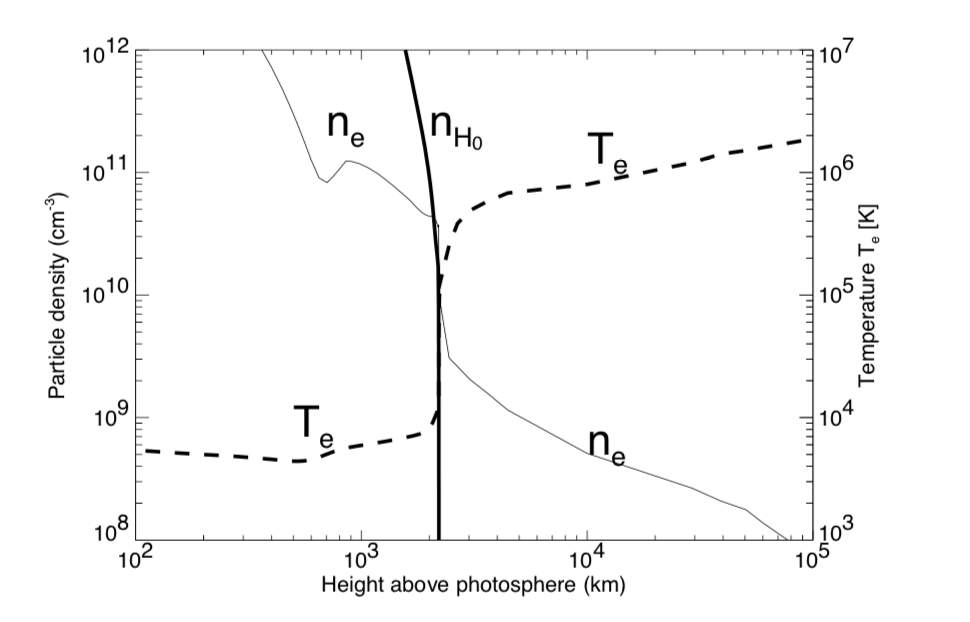
\includegraphics[width=\columnwidth]{Images/Corona_temp.png}
    \caption[Model of electron density and temperature with height in the solar atmosphere.]{Model of electron density and temperature with height in the solar atmosphere. The x axis shows height above the chromosphere in kilometres while the y axes show particle density in cm$^{-3}$ and temperature in Kelvin. The chromosphere begins $\sim 500$~km above the photosphere. The region around 2000 km showing a sharp rise in temperature and sharp fall in electron density is known as the transition region. Above this height plasma becomes fully ionised and is known as the corona. Image from \cite{Aschwanden2004}.}
    \label{fig:corona_temp}
\end{figure}
%Figure \ref{fig:Sun} shows the interior layers of the Sun and its atmosphere.
%\begin{figure}[t]
%    \centering
%    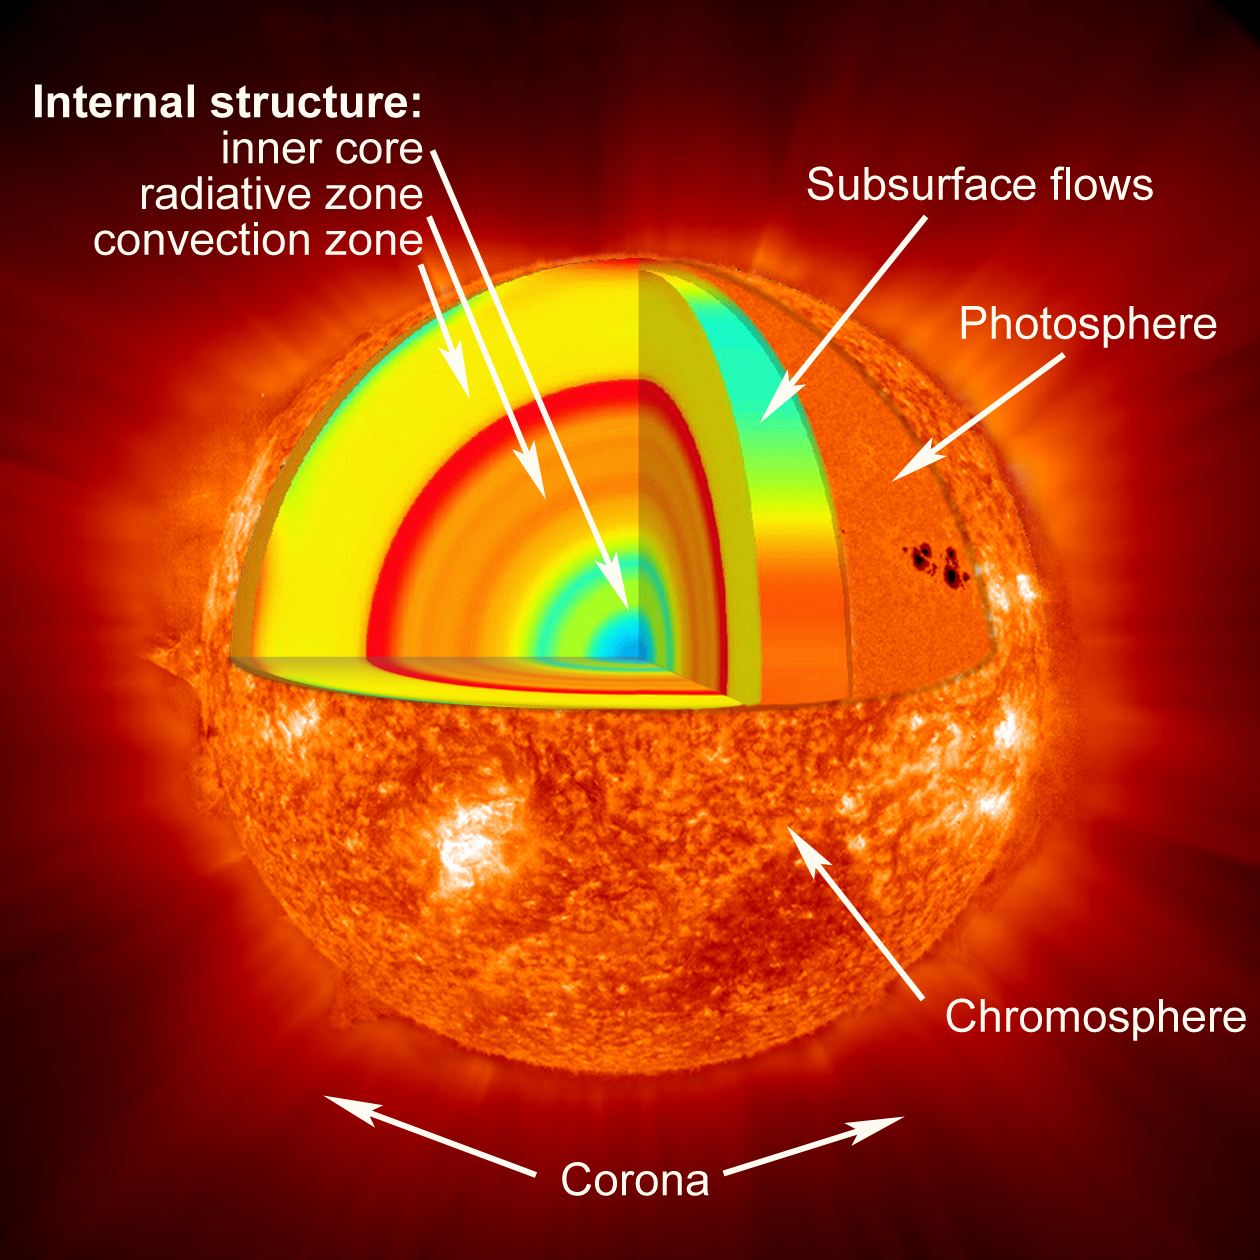
\includegraphics[width=0.5\columnwidth]{Images/Sun_interior.jpg}
%    \caption[Diagram of Sun's interior and atmospheric layers.]{Diagram of Sun's interior and atmospheric layers. Photons produced by nuclear fusion in the core transfer energy outwards through the radiative zone to ~0.7 R$_{\odot}$. At this point, convection becomes the main form of energy transport. The visible surface of the Sun is known as the photosphere and marks the boundary between the interior and the atmosphere. The solar atmosphere consists of three layers, the chromosphere, the transition region (not shown) and the corona.}
%    \label{fig:Sun}
%\end{figure}

\subsection{The Chromosphere}
In traditional plane-parallel models, the Chromosphere extends to $\sim 2000$ km above the photosphere. Its name is derived from the Greek word for colour, $\chi \rho \omega \mu \alpha$ (\textit{chroma}), in reference to the red coloured rim visible during solar eclipses. This red colour originates from the dominant Hydrogen-$\alpha$ (H$\alpha$) transition at 656.3 nm. Temperatures in the chromosphere show a decrease with distance to a local minimum of $\sim 4400$ K at $\sim 500$ km above the photosphere. The temperature then rises again to a maximum of $\sim 20,000$ K at its upper boundary. These temperatures are low enough that most of the hydrogen in the chromosphere remains neutral. 

The chromosphere exhibits numerous structures and dynamics often observed in emission lines such as H$\alpha$, the Ca II H and K lines and the Lyman-$\alpha$ transition of Hydrogen. The most prominent structural features of the quiet chromosphere include the chromospheric network on the disk and small, almost ubiquitous, jets of plasma known as spicules on the limb. The chromospheric network forms along the boundaries of supergranular cells where magnetic fields are concentrated. The magnetic field strength in the network can reach hundreds of millitesla although the average field strength of the chromosphere is $\sim 3$~mT \citep{McLean1985}.

% have been observed and are theorised to be a contributor to coronal temperatures.
% These are almost all due to the flux emergence of magnetic field in the chromosphere as evidenced by the supergranular structure. S

\subsection{The Transition Region}
The transition region occurs between the chromosphere and corona. Rather than a geometric layer, it is more accurate to consider the transition region as the region where the temperature rapidly increases (over distances as short as $\sim 100$ km) from $\sim 20,000$K to $\sim 0.8$ MK. Because the pressure remains approximately constant over this distance, the electron number density drops dramatically as is shown in Figure \ref{fig:corona_temp}. The transition region is also the part of the solar atmosphere where plasma changes from being partially ionised and collisionally dominated to fully ionised and collisionless. Network structures are also visible in low transition region images and are generally larger than those of the chromosphere, suggesting an expansion of magnetic flux tubes with height. However, the network completely disappears in higher altitude images hence, the magnetic field structure transitions from being ordered in the chromosphere to being extremely complex in the corona \citep{Tian2017}. Emission from the transition region is predominantly in the ultraviolet and extreme ultraviolet.

\subsection{The Corona}
The outermost layer of the solar atmosphere is called the corona. It contains hot, tenuous, inhomogeneous and time varying plasma which extends from the top of the transition region into interplanetary space.
%which displays a number of interesting phenomena thought to be governed by its complex magnetic field. The corona begins $\sim 2500$ km above the photosphere after a layer in the Sun's atmosphere known as the transition region, where electron density decreases and temperature increases dramatically (Figure \ref{fig:corona_temp}). 
The electron density in the corona ranges from $10^{9} \mbox{ cm}^{-3}$ at the base to $10^{6} \mbox{ cm}^{-3}$ at distances of 1 R$_{\odot}$ from the solar surface. Densities vary throughout the corona. Sparse, underdense regions at the base of the corona known as coronal holes exhibit densities of $\sim ( 0.5 - 1.0) \times 10^8 \mbox{ cm}^{-3}$ whereas areas of high magnetic activity known as active regions have electron densities of $\sim 2 \times 10^9 \mbox{ cm}^{-3}$. Active regions are the coronal counter part to sunspots and are best seen in EUV images of the Sun. The complex magnetic fields in active regions drive many of the solar phenomena such as solar flares and coronal mass ejections (CMEs).
 %Certain areas in the corona however, exhibit electron densities approximately an order of magnitude greater than the ``quiet Sun". Theses areas of high electron densities ar 

Observing the white light corona is done with a number of ground-based and space-based instruments called coronographs, that emulate the effect of a total eclipse. The Large Angle and Spectrometric Coronagraph \citep[LASCO;][]{Brueckner1995} on board the Solar and Heliospheric Observatory (SOHO) is one such instrument and allows the corona to be observed from distances of 2-32 R$_\odot$. The corona is also observed in extreme ultraviolet (EUV) lines, soft X-rays and at radio wavelengths. Observations at various wavelengths show a plethora of structure in the corona both on disk and on the limb that exist on varying time scales of a few minutes to a number of days. All particle acceleration events that produce radio emission of interest to this thesis occur in the solar corona. Figure \ref{fig:aia_quad} shows the corona and other layers of the solar atmosphere observed with the Atmospheric Imaging Assembly \citep[AIA;][]{Lemen2012}.

The high temperature of the corona remains one of the greatest mysteries in all of solar physics. Energetic events in the corona such as solar flares and CMEs, described in \ref{subsec:sf} and \ref{subsec:CMEs}, are observed across the electromagnetic spectrum. They are studied in order to understand how particles are accelerated, how energy is released and ultimately, why the corona has such an unaccountably high temperature.

% have a diagnostic in radio spectra. This PhD focuses on studying these radio diagnostics at their highest temporal and spatial resolutions to date.
\begin{figure}[ht]
\centering
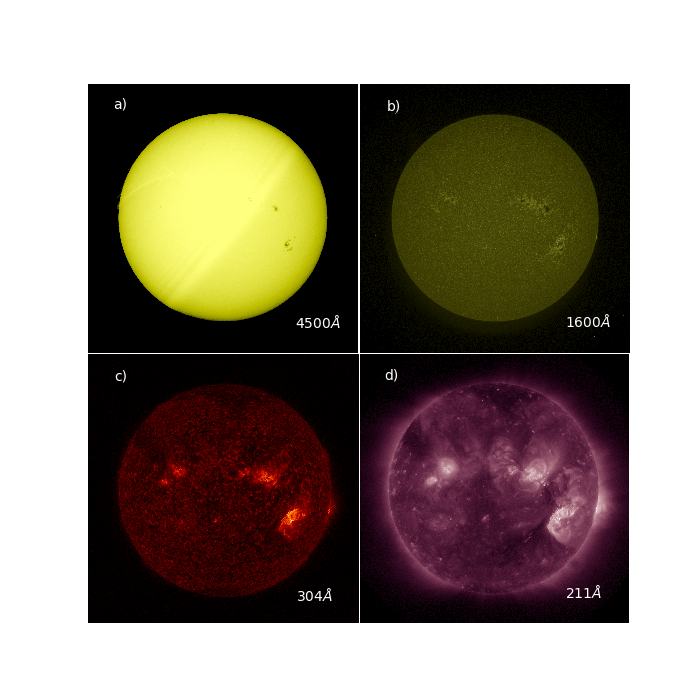
\includegraphics[width=0.8\columnwidth]{pm_aia_quad.png}
\caption[The solar atmosphere at different wavelengths.]{The Sun observed with AIA in four different wavelengths. Panel a shows the photosphere at 4500{\AA}, a group of sunspots is visible towards the southwestern limb of the sun. Panel b shows the chromosphere at 1600{\AA} and exhibits the chromospheric network. Panel c shows the upper chromosphere and transition region at 304{\AA}. Panel d shows the upper corona at 211{\AA} the active region is noticeable as the bright region in the same location as the sunspot group as in panel a.}
\label{fig:aia_quad}
\end{figure}

\section{Solar Flares}
\label{subsec:sf}
Solar flares are massive releases of magnetic energy commonly believed to be due to a reconfiguration in the complicated magnetic field structure in an active region.  They are some of the most energetic events in the solar system, releasing $\sim 10^{25}$ J of energy over a matter of minutes. Flares are observed across the electromagnetic spectrum from radio waves to $\gamma$ rays with energies $> 10$ MeV. They are classified by the amount of X-ray flux (W m$^{-2}$) detected by the Geostationary Operational Environmental Satellite (GOES) 1-8 {\AA} band on a logarithmic scale as being A, B, C, M or X class with A being the lowest flux ($10^{-8} \mbox{ W m}^{-2}$) and X the highest ($10^{-4} \mbox{ W m}^{-2}$). Each class is further subdivided into a linear scale.
A timeseries of X-ray flux from a solar flare is often called a lightcurve and has three characteristic phases; a pre-flare phase which shows X-ray flux associated with the active region where the flare occurs, an impulsive phase showing a sharp rise in X-ray flux corresponding to accelerated particles colliding with the solar surface, and a gradual decay phase where plasma heated by the flare gradually cools back to its pre-flare state. Figure \ref{fig:GOES_Xclass} shows a GOES light curve of the X9 class flare that occurred on 10 September 2017 and the three flare phases described above.

\begin{figure}[ht]
    \centering
    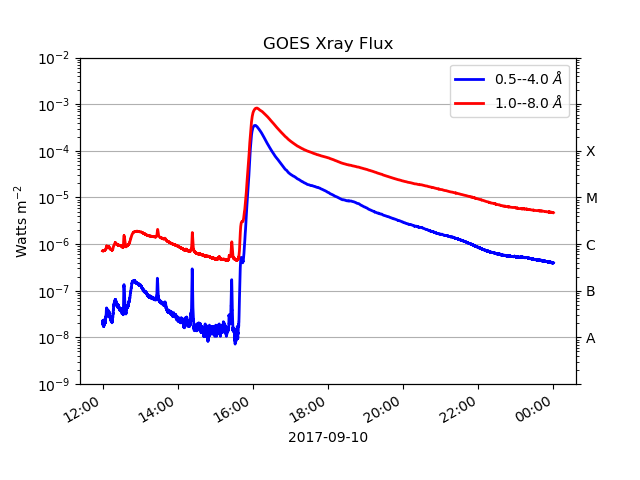
\includegraphics[width=\columnwidth]{Images/GOES_Xclass.png}
    \caption[GOES lightcurve for X9 class flare on 10 September 2017.]{The GOES lightcurve of the X9 flare that occurred on 10 September 2017. The x axis indicates the time of day on 10 September 2017 while the y axes show the X-ray flux in Wm$^{-2}$ and the flare classification. The red curve shows the 1-8 {\AA} channel by which the flare is classified while the blue curve shows the 0.5-4 {\AA} band. The three characteristic phases of a solar flare are clearly displayed here. The pre-flare phase before $\sim$ 16:00 UTC, the impulsive phase indicated by the sharp rise in flux and the gradual decay phase where X-ray flux gradually returns to the pre-flare level.}
    \label{fig:GOES_Xclass}
\end{figure}
During solar flares, magnetic structures known as coronal loops fill with hot plasma and begin to emit in soft X-rays. At the same time, electrons are accelerated towards the solar surface where their energy is converted to hard X-rays in the collision via bremsstrahlung. 

\section{Coronal Mass Ejections (CMEs)}
\label{subsec:CMEs}
In certain magnetic reconnection events, plasma suspended in a magnetic flux rope erupts from the corona into the heliosphere, the volume around the Sun where the interplanetary medium is dominated by particles flowing outward from the Sun. These eruption events are known as coronal mass ejections and accelerate 10$^{15}$ g of charged particles at typical speeds of up to $\sim 2500 \mbox{ km s}^{-1}$ \citep{Gopalswamy2000}. A ``textbook" CME structure consists of a bright front that surrounds a dark cavity and a bright central core. CMEs are observed using coronographs as they are much fainter than the solar disk. An example of a CME observed using the LASCO C2 corona with a field of view from 1.5 R$_\odot$ to 6 R$_\odot$ can be seen in Figure \ref{fig:CME}. Ejected material from a CME can interact with the Earth's magnetosphere and are known to have caused adverse effects including satellite communication disruption, radio blackouts, wide spread power outages and large inaccuracies in GPS postions \citep{Eastwood2017}. CMEs can travel faster than local Alfv\'{e}n speed in the corona leading to a shock which can accelerate particles. 

\begin{figure}[ht]
    \centering
    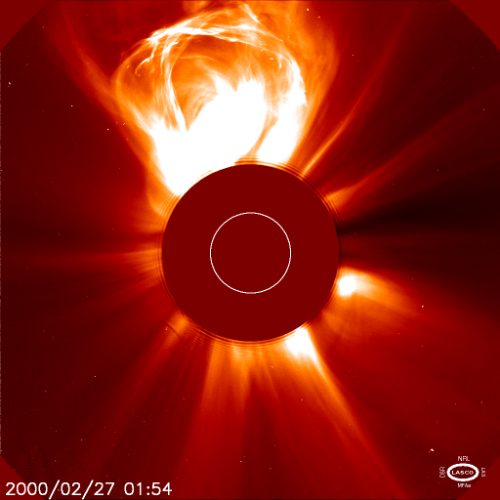
\includegraphics[width=0.75\columnwidth]{Images/LASCO_C2_CME.jpg}
    \caption[CME observed with the LASCO C2 coronograph on 27 February 2000.]{A coronal mass ejection (CME) observed with the LASCO C2 coronograph on 27 February 2000. The area covered by the coronograph is shown in the red disk in the centre of the image and the white circle represents the solar disk. The bright feature in the top of the image is the CME while less bright structures known as streamers are also seen.  }
    \label{fig:CME}
\end{figure}

\section{Solar Radio Bursts}
\label{sec:solar_radio_bursts}
In 1942 while Britain was monitoring radar signals for the signs of enemy aircraft, a strong, noise like and highly variable signal was noticed by radar operators. Upon investigation it was found that this jamming was in fact radio emission from the Sun. The discovery of this radio emission being associated with a major solar flare was kept secret until after the war and was published by \cite{Appleton1946}.
Since then the field of solar radio astronomy has flourished and significant advancements in both instrumentation and theory have occurred. Worldwide, radio interferometers such as the LOw Frequency ARray \cite[LOFAR;][]{VanHaarlem2013} and the Murchison Widefield Array \citep[MWA;][]{Lonsdale2009} have been built while next generation interferometers like the Square Kilometre Array \citep[SKA;][]{McMullin2020} are slowly being brought online. These telescopes offer a dramatic improvement on the spectral resolution and imaging capability of those that were first used to study solar radio emission.

Solar radio emission often comes in the form of bursts of varying time scales. These were initially classified into three types by \cite{Wild1950b} with a fourth and fifth type being discovered by \cite{Boischot1957} and \cite{Wild1959} respectively. A wealth of other fine structure radio bursts are also observed, predominantly found in radio storms such as S bursts, drift pairs and stria \citep{McConnell1980,Melrose1982,NelsonandMelrose1985}. 
The fine structure of these bursts can often reveal information about small-scale turbulence in the corona \citep{Reid2021}.
Figure \ref{fig:burst_cartoon} shows a schematic of the five ``classic" types of solar radio burst. A brief description of some solar radio phenomena is given below.
\begin{figure}[ht]
    \centering
    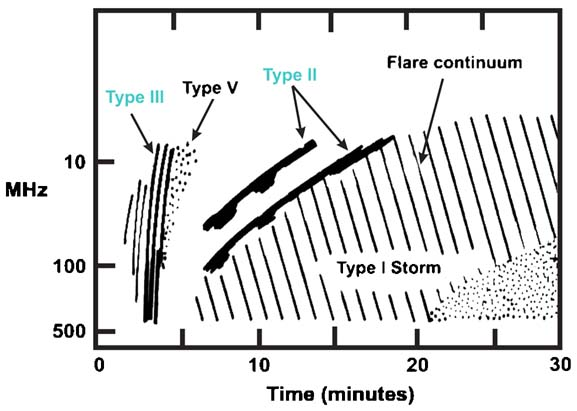
\includegraphics[width=0.75\columnwidth]{Images/Burst_cartoon.jpg}
    \caption[Cartoon of type I-V radio bursts.]{A cartoon of type I-V radio bursts. The x axis shows the time scale of the various bursts which can range from less than 1 minute to greater than 10 minutes. The y axis shows the typical frequency range of the bursts. The different drift rates of the different burst types are apparent. Image from \cite{Cliver2009}.}
    \label{fig:burst_cartoon}
\end{figure}
\paragraph{Type I bursts}
Type I emission can appear as bursts and/or a continuum originating from ``storm centres" that are associated with active regions. Type I storms can last for many days. Emission from type I bursts is highly circularly polarised in the o-mode (whereby light is circularly polarised in the opposite direction as electrons gyrating about a magnetic field line) and is also particularly directional with an increase in intensity as active regions rotate to the centre of the disk. Unlike type II or III bursts, they do not exhibit a harmonic structure \citep{McLean1985}.
\paragraph{Type II bursts}
Type II radio bursts are a form of radio emission seen from the Sun and are identified by a slow ($\sim 0.1$~MHz~s$^{-1}$) drift to lower frequencies in dynamic spectra. The frequency drift can be used to find the velocity of the shock causing a burst if the electron number density as a function of height is known. The velocities of type II bursts are often found to be $\sim 1000 \mbox{ km s}^{-1}$, which is faster than the Alfv\'{e}n velocity in the quiet corona meaning a shock must be present \citep{NelsonandMelrose1985}. Other basic properties of type II bursts include:
\begin{enumerate}
    \item Narrow bandwidths of up to $\sim 100$~MHz from initial to final frequencies.
    \item A harmonic structure of two bands with a frequency ratio slightly less than 2:1 at a fundamental, $f_p$, and harmonic, $2f_p$, frequency can be seen for most type II bursts. This structure is consistent with the idea that type II emission is due to plasma oscillations.
    \item A large number of type II bursts contain band splitting into an upper and lower band for each of the harmonics in their spectra. The cause for this splitting is not fully understood but it is commonly thought that the two bands are related to emission upstream and downstream of the MHD shock front which causes the type II burst \citep{Smerd1974,NelsonandMelrose1985, Vrsnak2002}.
    \item Herringbone structure. Approximately 20\% of type II bursts show a herringbone structure of rapidly drifting emission spikes shooting out of the ``backbone" of the main frequency drift to higher and lower frequencies. These herringbones are thought to be due to electron beams being accelerated at the associated shock for the type II burst \citep{Mann1995}. While the backbone is poorly polarised, the herringbones have been found to be quite strongly, $\sim 70\%$, polarised. The level of polarisation of herringbones determined by \cite{Suzuki1980} are similar to those of type III bursts. They suggest that this is evidence that herringbone structure is due to plasma emission from accelerated electron beams such as in the case of type III bursts. 
    \item Starting emission frequencies of the order of a few 100~MHz ending at frequencies above 20~MHz. This being said, type II burst with starting frequencies of $\sim 100$ kHz have also been observed. 
    These lower frequency bursts are thought to be due to interplanetary shocks whereas higher frequency bursts are considered to be from shocks in the low corona.
    \item Typical durations of 5-15 minutes. type II bursts that occur after a flare do so with a delay ranging from 2-20 minutes. Bursts with shorter durations generally have higher starting frequencies. %Timing and duration    
\end{enumerate}
 
Based on these and a number of other properties discussed in greater detail by \cite{NelsonandMelrose1985}, type II radio bursts can be used as indicators for MHD shocks in the solar corona. Observational proof of frequency varying inversely with time in the solar wind, consistent with radiation being generated at $f_p$ and $2f_p$ directly upstream from a CME-driven shock, was found by \cite{Reiner1997} and solidifies this argument.
\paragraph{Type III burst}
Observations of type III radio bursts (and their sub-categories) are of particular interest to this thesis and, as such, are described in Section \ref{sec:typeIII}.
\paragraph{Type IV burst}
Type IV bursts come in at least three sub-types with the general characteristic that they are of the from of broadband emission lasting for several hours. Early stationary type IV bursts (also known as the flare continuum) associated with the decay phase of solar flares, late stationary bursts which appear similar to type I emission, and moving type IV bursts which exhibit a smooth, wide-band spectrum \citep{McLean1985}.
\paragraph{Type V burst}
The last of the broadband emission bursts, type V radio bursts typically have a duration of 1-3 minutes and appear as an afterglow from type III bursts. Type V emission is strictly less than 150~MHz and is accepted that it results from electrons that generate a type III burst and become trapped in a closed magnetic loop in the corona \citep{McLean1985}.

\paragraph{Fine Structure: S bursts} 
S bursts, initially called Fast Drift Storm (FDS) bursts, were first observed at the Culgoora Solar Observatory in 1967 \citep{Ellis1969} They were later renamed by \cite{McConnell1980} who likened them to Jovian S bursts. They have a narrow bandwidth of the order of 0.03~MHz and a drift rate of 1-2~MHz~s$^{-1}$ and durations much less than 1s. \cite{McConnell1980} also concluded that S bursts are radiated at either the plasma frequency or its harmonic in a manner similar to type III bursts but that the implications of S burst fine structure and coronal scattering can only be defined once it is determined which harmonic of the plasma frequency they are radiated at. \cite{Melnik2010} propose a model of S bursts being generated by coalescence of fast magnetosonic waves with Langmuir waves which agrees well with the analysis of \cite{Clarke2019}. Modern observations of S bursts, such as those conducted using LOFAR's tied-array imaging mode \citep{Morosan2015}, can give greater insight into the spectral and temporal variability of S bursts and what this might mean for the environment they are generated in.
\\
\\The spatial extent and fine spectral structure of type III radio bursts are the main focus of this thesis. In Section \ref{sec:typeIII} below I outline the physical characteristics of type III bursts and their subcategories.

\subsection{Type III Bursts}
\label{sec:typeIII} 
Type III bursts are possibly the most useful radio burst for studying properties of plasma in the corona. As we shall see, they offer a remote measurement of the plasma density of the region where they are emitted. This allows us to probe the solar corona plasma using any of the many radio telescopes on Earth dedicated to solar radiophysics \citep[e.g.][]{Benz2004}.
\cite{Reid2014} review the observational properties of type III bursts which are repeated in brief here. The defining characteristic of type III bursts is a drift from high to low frequencies in a dynamic spectrum. The drift rates for type III bursts are typically quite fast, of the order of $\sim$ 10~MHz~s$^{-1}$ depending on the frequency. The frequency drift rate, $df/dt$, has been found to have various relations with frequency \citep{Reid2014} but most agree that $df/dt \propto f^{\alpha}$, where $\alpha$ ranges in the literature from $\sim 1$ to $\sim 2.7$. 

\cite{Ginzburg1958} proposed that type III bursts are emitted at the plasma frequency,
\begin{equation}\label{eq:1}
    \omega_{p}^2 = \frac{N_e e^2}{m_e \varepsilon_0}
\end{equation}
where $N_e$ is the number density of electrons, $m_e$ is the electron mass, $e$ is the electron charge and $\varepsilon_0$ is the permittivity of free space. A more detailed description of the plasma emission process is given in Section \ref{sec:plasma_emission}.
Although Eq. \ref{eq:1} is relatively simple, it contains an important relationship in plasma physics. Namely, the plasma frequency is proportional to the square root of the electron density. This means that plasmas at higher electron densities will oscillate at higher frequencies than those of lower densities. The drift in type III bursts, which are emitted at $\omega_p$, is therefore an indication of the emission source moving from an area of high electron density to low density, i.e. from the lower to the upper corona. Using a model of electron density in the corona such as the \cite{Newkirk1961} model, it can be inferred that the exciter of type III bursts has a speed of $\sim 0.3$~c.

\begin{figure}[ht]
    \centering
    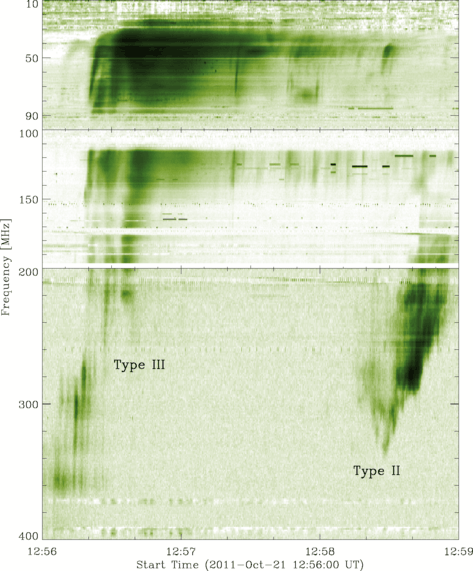
\includegraphics[width=0.75\columnwidth]{Images/Pietro_typeIII.png}
    \caption[A number of type III bursts observed by \cite{Zucca2012} on 21 October 2011.]{A number of type III bursts observed by \cite{Zucca2012} on 21 October 2011. The x axis gives the time on 21 October 2011 while the y axis shows the frequency in MHz. A number of type III bursts extend to frequencies below 200~MHz. A type II burst can be seen between 140 and 330~MHz later in the day.}
    \label{fig:bursts}
\end{figure}

Type III bursts are observed to be in two bands, a fundamental and harmonic band that are emitted at $\omega_p$ and $2 \omega_p$ respectively. Both bands exhibit the same frequency drift although the flux of the harmonic band is usually less than that of the fundamental band \citep{Wild1954a, McLean1985}. The process of plasma emitting radio frequencies at $\omega_p$ and $2 \omega_p$ will be explained in more detail in Chapter \ref{chap:theory}. 
Figure \ref{fig:bursts} shows type III radio bursts below 400~MHz observed by \cite{Zucca2012}. A type II burst was also observed between 140 and 330~MHz and exhibits a much slower frequency drift than the type III bursts. A type III storm can be seen below 200~MHz. This is when type III emission is continuous over the span of large time scales and can last days. Type III bursts come in a number of subcategories described below.

\paragraph{Reverse and bi-directional bursts.}

A typical type III burst is produced when an electron beam travels along a magnetic field line away from the Sun to areas of lower density. If, instead, electrons travel towards the Sun to areas of higher density a reversed frequency drift is observed. Bursts where both the regular and reverse drifts can be seen simultaneously are bi-directional bursts \citep{Reid2014}.

\paragraph{Type IIIb bursts.}

\begin{figure}[ht]
\centering
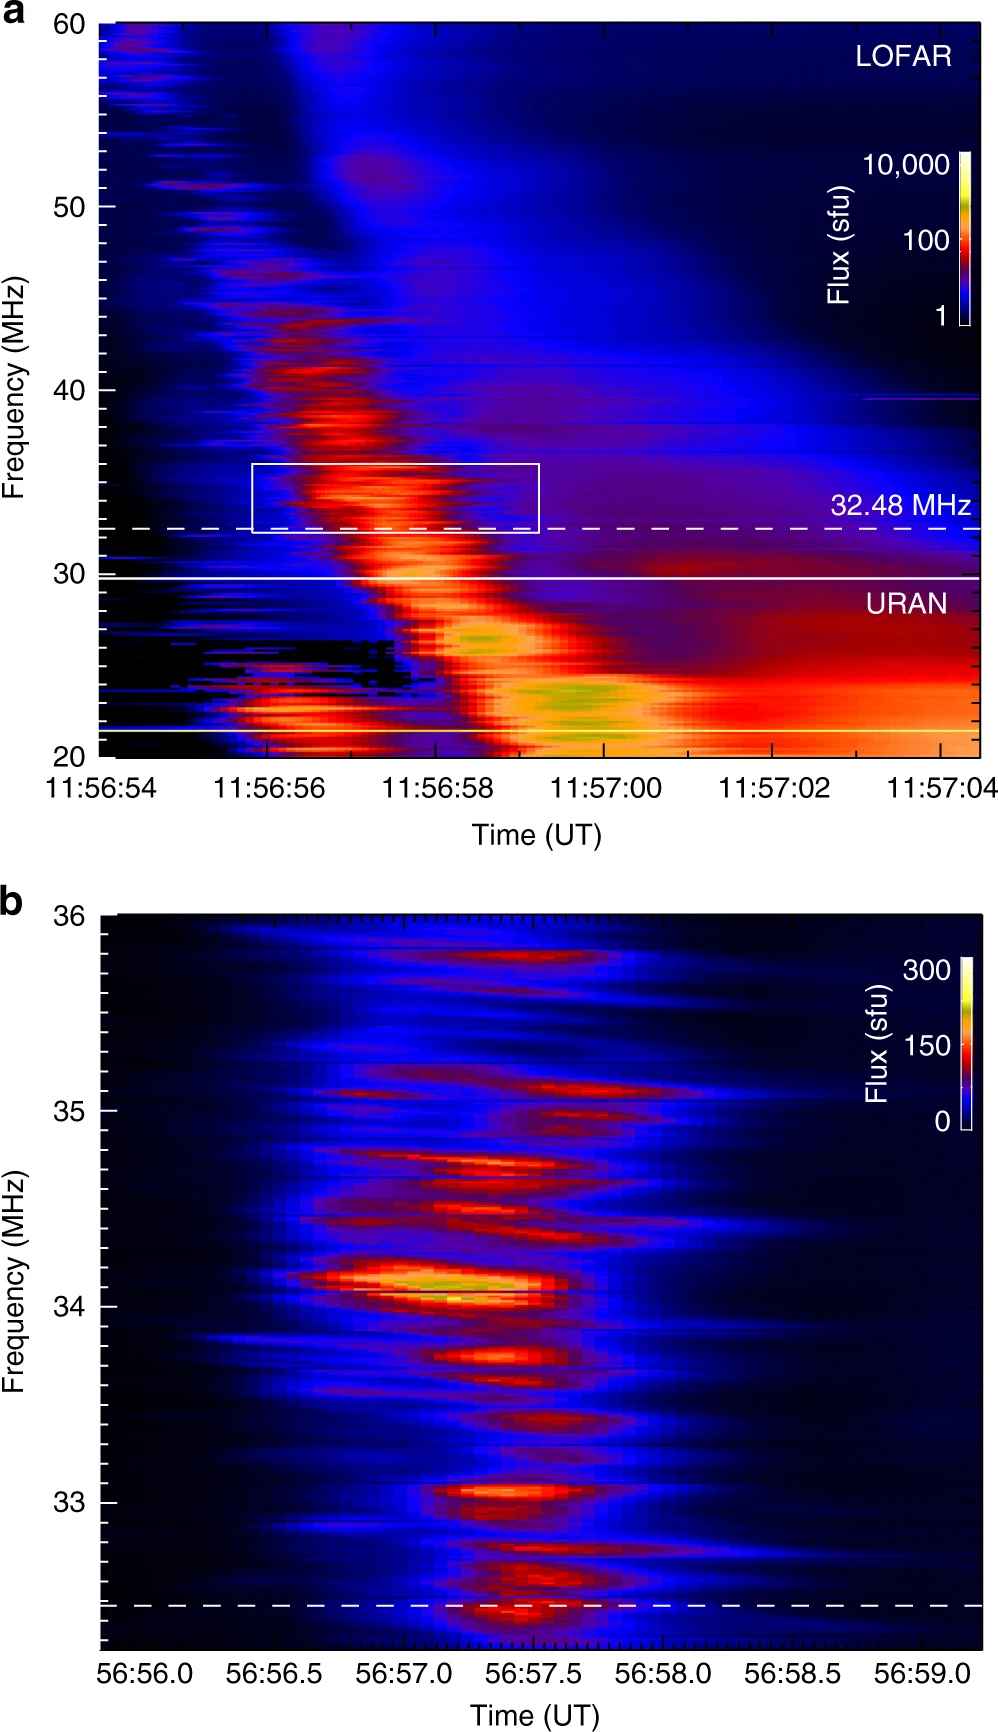
\includegraphics[width=0.5\columnwidth]{typeIIIbKontar.png}
\caption[The type IIIb radio burst from \cite{Kontar2017}.]{A type IIIb radio burst on 16 April 2015 analysed by \cite{Kontar2017}. Panel a shows the full duration of the type IIIb. Panel b is a zoom in of the 3 second wide box in panel a.}
\label{fig:typeIIIbKontar}
\end{figure}

Fine frequency structures are sometimes seen in type III bursts. Type IIIb radio bursts are defined as a number of narrow, nearly horizontal, frequency bands called striae, or striations, in the envelope of a type III. The frequency width of an individual striae is typically 0.05~MHz \citep{McLean1985} and they have a frequency drift rate of $\lesssim 150$~kHz~s$^{-1}$, which implies a speed of 0.6~Mm~s$^{-1}$ \cite{Sharykin2018}. Figure \ref{fig:typeIIIbKontar} shows a dynamic spectrum of a type IIIb burst from \cite{Kontar2017}. Individual striae can be clearly seen in panel b of Figure \ref{fig:typeIIIbKontar}. The theory describing the origin of this fine frequency structure has recently been revisited by \cite{Reid2021} who found that the striations are due to turbulence in the corona and their drift a result of moving Langmuir waves.

\paragraph{Type U and J bursts.}

In the case where electrons are travelling along a closed magnetic field line, a turning point in the frequency drift of a type III burst can be observed. For electrons that generate radio emission down to the footpoint of the magnetic field line, a U burst is observed. A U burst can be identified as an inverted U on a dynamic spectrum. More often, electrons stop generating radio emission as they travel back down the magnetic field line so only the turning point in frequency drift is visible in dynamic spectra. These are known as J type bursts. U and J bursts are far less common than type III bursts, despite the similar number of open and closed magnetic field lines along which electron beams can propagate. The reason for this proposed by \cite{Reid2017} is that the length of these closed loops is not long enough for the electron beam to become unstable to Langmuir waves.

\paragraph*{} The study of type III bursts offers an insight into the process of Langmuir wave generation in the solar corona and as such are an important tool in understanding the physics of coronal plasma \citep{Reid2014}. However, the effects of radio wave propagation from the source to the observer through the corona must but understood before inferences can be drawn from observations. 

\subsection{Low Frequency Radio Wave Scattering}

Spectral analysis of short temporal radio bursts with small bandwidths at $\sim 30$~MHz suggests that source sizes in the corona are of the order $\lesssim 1$ arcmin \citep{McConnell1980, Kontar2017}. Radio images of the Sun at metric and decametric wavelengths have yet to reveal this level of spatial structure. This was mostly due to the limitations of angular resolution of radio telescopes at the time. 
Observations with modern interferometers at these frequencies however, still have not observed spatial structure at these scales. The suggestion that there is a fundamental limit imposed upon the level of resolution obtainable by scattering of radio waves in a turbulent corona \citep{Bastian1994} has re-emerged in recent years \citep{Thejappa2007,Thejappa2008,Kontar2017,Kontar2019}. 

The development of scattering theory stems from \cite{Chandrasekhar1952} description of light scattered by a thin screen and will be outlined further in Chapter \ref{chap:theory}. The implementation of this theory into computational modelling has also seen considerable development since the first ray tracing experiments by \cite{Fokker1965}. \cite{Steinberg1971} built upon this by including the effect of spherical refraction through the corona and were able to obtain the time response of a scattered pulse source.

Both \cite{Fokker1965} and \cite{Steinberg1971} followed from \cite{Chandrasekhar1952} and assumed density inhomogeneities in the corona had a Gaussian power spectrum. However, it is now known that this assumption is incorrect. \cite{Bastian1994} provides a review of the work by \cite{Coles1989} and others to determine the shape of density inhomogeneity power spectrum. At large scales, greater than a few hundred kilometres, the spectrum is well described with a power law index of 11/3, which agrees with the Kolmogorov description of turbulence \citep{Kolmogorov1941}. For scales smaller than these but greater than a few kilometres, the spectrum becomes shallower and is better described with a power law index of $\sim 3$. Finally, on the smallest scales less than a few kilometres the spectrum steepens again. This steepening has been interpreted as the scale at which energy is dissipated by turbulence. \cite{Coles1989} also found that this inner scale increases with heliocentric distance. \cite{Bastian1994} expanded on this description of the density inhomogeneity power spectrum and investigated the angular broadening of radio waves sources at centimetre wavelengths.

The latest development in the modelling of radio wave scattering is by \cite{Kontar2019}. Rather than using the small scattering angle approximation of previous work, \cite{Kontar2019} build on the work of \cite{Arzner1999} and \cite{Bian2019}. In this approach, the effect of anisotropic density inhomogeneities is treated as photon diffusion in momentum space and the Hamiltonian equations for photon position and momentum can be solved iteratively to trace a photon's path. This allows for a continuous transition from weak to strong scattering, whereas previous work is limited to regime of small angle scattering. 

Understanding radio wave propagation effects, in particular scattering, is important because they affect all observations made at radio wavelengths. Radio wave scattering has been shown to depend on the relative level of density fluctuations in the corona and as such, offers a chance to learn about its turbulent nature. By classifying the power spectral density of these fluctuations it may be possible to gain an understanding of the turbulent processes that transport energy to the microscopic scales and result in the heating of the corona. 

\section{Thesis Outline}
The high spatial, temporal and spectral resolution of modern radio interferometers such as LOFAR and the launch of new space missions including Parker Solar Probe \citep[PSP;][]{Fox2016} and Solar Orbiter \citep{Muller2020} has ushered in a new age of solar radio observations. By developing a computational backend and using a unique method for fitting interferometric visibilities, this thesis has furthered the capability of an international LOFAR station and extracted value from existing interferometric observations. This thesis outlines how such developments have improved our knowledge of radio wave propagation in the solar corona using observations at some of the highest spatial, spectral and temporal resolutions available. In Chapter \ref{chap:theory} I outline the relevant background theory for the work presented in this thesis. Chapter \ref{chap:instrumentation} will describe the instrumentation used throughout this thesis, namely LOFAR, and the mathematical background for interferometric imagining. 

The REALtime Transient Acquistion backend (REALTA), is a seven node computer cluster designed to record and analyse the raw beamformed data from international LOFAR stations in real-time. The development of REALTA for solar and a myriad of other observations formed a key part of this work. Chapter \ref{chap:REALTA} describes the hardware and software of REALTA and showcases some first light observations.
 
The study of radio wave scattering in the solar corona has undergone a renaissance in recent years both in terms of computational modelling and observations. Chapter \ref{chap:measuring_source_sizes} will describe how, for the first time, LOFAR visibilities were fitted directly to determine the size and position of a type IIIb burst. This lead to a more subtle understanding of the root mean squared fluctuations of electron density in the solar corona, the key parameter necessary to quantify the effect of scattering. 

In order to accurately compare between models of the solar corona, in Chapter \ref{chap:observations_vs_theory} I present 29 type III radio bursts and determine their size and position using the visibility fitting technique with a Markov Chain Monte Carlo optimization. The results of this show that type III bursts exhibit an intrinsic source size greater than the size of a point source that has been scattered and highlights discrepancies between observations and computational modelling.

Chapter \ref{chap:future} includes a discussion on the future work that can be carried out from the foundations of this thesis. It outlines the necessary further studies needed to further our knowledge of radio wave scattering and how to utilise even higher temporal resolution observations of the radio sun. Chapter \ref{chap:future} will also contain a summary and conclusion of the work presented in this thesis.

	
%%!TEX root = ../main.tex
%Adding the above line, with the name of your base .tex file (in this case "thesis.tex") will allow you to compile the whole thesis even when working inside one of the chapter tex files
%%
%%
\onehalfspacing
\chapter{Instrumentation}
\label{chap:inst}
\section{LOFAR: The LOw Frequency ARray}
The LOw Frequncy ARray (LOFAR, \citeauthor{VanHaarlem2013b} \citeyear{VanHaarlem2013b}) is a radio interferometric array spread across Europe. The first LOFAR core station was completed in 2008. Since then, LOFAR has continued to grow to 38 stations in the Netherlands alone with a further 13 across the rest of Europe and 2 more stations planned for completion in 2019/20. Along with the addition of new stations, an extensive set of software for imaging, calibration, RFI flagging and more has been written for use with data produced by LOFAR. Imaging pipelines described in \cite{VanHaarlem2013b} have also been developed to further maximise the quality of the sub-arcsecond spatial resolution data LOFAR can provide with its full $\sim 2000$ km baseline.
Every LOFAR station is connected to the CEntral Processor cluster (CEP) located in Groningen in the Netherlands by 10 Gbps fibre optic cable where data is beamformed and correlated by the COrrelator and Beamformer Application for the LOFAR Telescope (COBALT), a GPU based cluster using commercial components \citep{Broekema2018}.

LOFAR observes radio electromagnetic radiation at frequencies of 10-240MHz in two bands, 10-90MHz and 110-240MHz. The gap between the two bands is included in order to avoid observing in the noisy FM band which is dominated by commercial radio broadcasting. To observe in each band, two different antenna designs are utilised, the Low Band Antenna (LBA) for 10-90MHz and the High Band Antenna (HBA) for 110-240MHz. Both are designed to use highly available, and thus moderately cheap, construction material such as PVC pipe or wire mesh. % In order to observe in these two bands, LOFAR uses two different antenna designs, the Low Band Antenna (LBA) for 10-90MHz and the High Band Antenna (HBA) for 110-240MHz.
Data recorded from the HBAs and LBAs is sampled at 200 MHz and channelised to 512 subbands by the Remote Station Processing (RSP) boards resulting in a temporal resoultion of 5.12 $\mu$s. Data can be stored temporarily at its full 5 ns resolution using the Transient Buffer Boards.
The hardware and electronic components of a LOFAR station are described below and are shown in the context of the digital signal processing path for a LOFAR station in Single Station Mode in Figure \ref{fig:sig_pipe}.
\begin{figure}
    \centering
    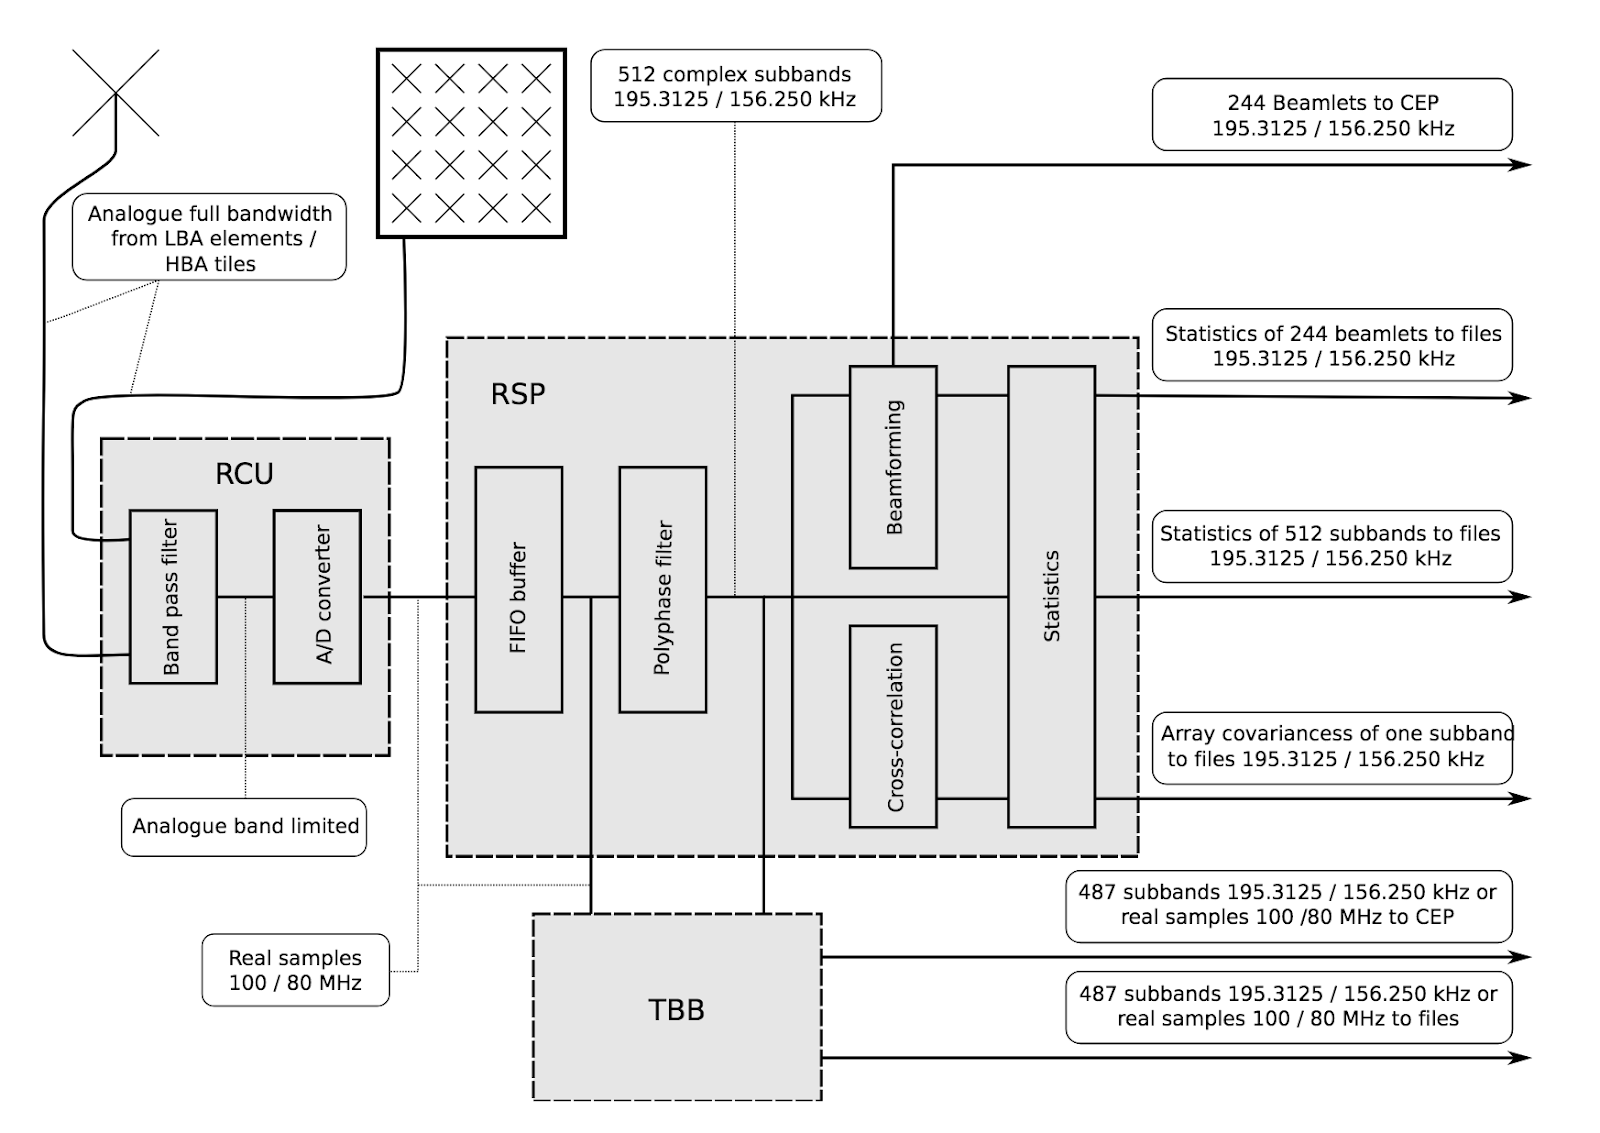
\includegraphics[width=0.75\columnwidth]{Images/Digital_signal_processing.png}
    \caption[Digital signal processing pipeline of an individual LOFAR station.]{Digital signal processing pipeline of an individual LOFAR station. Data is first digitised in the ReCiever Unit (RCU) before being sent to the RSP board. Here data is channelised by a polyphase filter and beamformed before being sent to the CEntral Processor (CEP) in the Netherlands. Also featured is the TBB which stores data in a ring buffer unless it is read out to an external storage system. }
    \label{fig:sig_pipe}
\end{figure}
\subsection{Low Band Antenna}
The LBA consists of two lengths of copper wire which act as a cross dipole antenna, allowing measurements from two linear polarisations. These are connected to a preamplifier placed on top of a PVC pipe. 
Each wire is 1.38 m long which results in a 52MHz resonance peak in power spectra: however, due to the impedance of the amplifier this is increased to 58MHz. A typical LBA power spectrum is shown in Figure \ref{fig:mode3_spec}.
\begin{figure}[t]
    \centering
    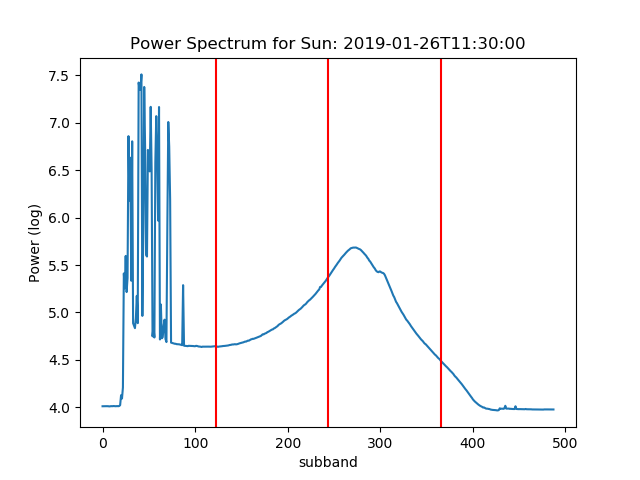
\includegraphics[width=0.75\columnwidth]{Images/Sun_pspec.png}
    \caption[Typical power spectrum for an LBA.]{Typical power spectrum for an LBA. Here the red vertical lines denote the sections of the spectra made from the different RSP lanes (Section \ref{sec:rsp}).}
    \label{fig:mode3_spec}
\end{figure}
The LBA is attached to a steel ground plane made out of concrete reinforcement rods by synthetic rubber straps and polyester rope. The ground plane acts as a reflector for radio waves, increasing the signal received by the antennas.
The simple design of the LBA and the fact that it observes at such low frequencies means that it is sensitive to the entire sky at once. Digital beamforming techniques are used to point an LBA array at a particular location on the sky, the direction of which can be changed in a manner of seconds.
%This pipe is anchored to a metal ground plane made out of steel commonly used in concrete reinforcement by two 1.38m copper wires which act as a cross dipole antenna, thus allowing both X and Y polarisations to be measured. The simple structure of the LBA means that there is a resonance peak at $\sim 58$MHz.
\subsection{High Band Antenna}
The higher frequencies LOFAR can observe at are recorded by the HBAs. The HBA design is drastically different to the simple design of the LBA so that system noise can be reduced. Each HBA is a 5 m $\times$ 5 m tile consisting of 16 bow-tie cross dipole antennae, all aligned in the same direction, supported in an expanded polystyrene structure. The HBA sits on top of a 5 cm $\times$ 5 cm wire mesh ground plane and is encased in two overlapping polypropylene foil layers in order to protect it from the weather. The finer mesh size in the ground plane for a HBA makes it more reflective for the $\sim 10$ cm waves being observed.% The majority of the tile is made out of expanded polystyrene making it lightweight and durable to weather condidtions. 
Each bow-tie antenna in a HBA tile is connected to a front-end which performs preamplification and analogue beamforming. Analogue beamforming is achieved using lengths of copper in a HBA front-end, the same digital beamforming techniques used for LBAs are also used for HBAs.
Each front-end is then connected to a summator where all the signals are summed before being sent for further signal processing in the station container (Section \ref{sec:sig_pipe}). 

\subsection{Remote Station Processing Boards (RSPs)}
\label{sec:rsp}
The RSPs perform all digital signal processing in a LOFAR station. Each LOFAR station consists of 24 RSP boards capable of channelising, beamforming and correlating raw voltage data recorded by either the LBAs or HBAs. A polyphase filter converts recorded data into 1024 complex subband signals which, because the signal is real, is fully described by the positive 512 subbands. These 512 subbands offer $\sim 195$ kHz frequency resolution across the observed band.
In order to perform beamforming, all RSPs are connected together in a ring. Data are passed along this ring and summed in each RSP where a phase correction is also applied in order to ``point" the telescope beam. A maximum of 488 subbands can be used to create beamlets, beams pointed in a particular direction observing in a particular frequency. Data from this process is streamed to an external storage node from 4 points in the ring along what are known as ``lanes" each containing one quarter of the beamlets computed by the RSP boards. 

%Access to the data from RSP boards directly is possible provided there is a sufficient computer back end and network setup capable of writing the data being sent at 3.3Gbps.
\subsection{Transient Buffer Boards (TBBs)}
\label{sec:tbb}
One of the lesser used pieces of LOFAR hardware are the Transient Buffer Boards (TBBs). TBBs are Random Access Memory (RAM) buffers that can temporarily store data at its natively sampled, 5 ns time resolution. Each LOFAR station contains a total of 12 TBBs ranging from 1 GB to 32GB of memory. More recently completed stations such as the Irish LOFAR station (I-LOFAR) have 32GB TBBs while the older Dutch stations usually have less than 16GB.
%A single TBB stores data from 8 different antennas with 2 polaristions each  
A 32 GB TBB can store up to 5 seconds worth of data recorded by a LOFAR station although this can be increased if fewer inputs or polarisations are recorded. TBBs are currently used in analysing cosmic ray showers and lightning storms but have yet to become a mainstream tool for solar physics, despite their potential. 
Recording the radio Sun at 5 ns has never been attempted before and could offer a wealth of never-before-studied phenomena or cast new light onto longstanding questions.

While the next generation telescopes like the Square Kilometre Array (SKA) and the Murchison Widefield Array (MWA) sample at higher rates than 5 ns, no other exisitng radio interferometer stores data at the sampled time resolution. This gives LOFAR the unprecedented ability to capture transient events at their highest temporal resolutions yet.

\section{I-LOFAR: The Irish LOw Frequency ARray}
One of the many benefits to using LOFAR as a radio telescope is that each station can be used independently in Single Station Mode which, in the case of international stations, gives freedom to the host countries to make specific observations that may not be covered in a LOFAR observing cycle. Not only this, but Single Station mode offers the flexibility of the raw complex voltage data before it has passed through any averaging or calibration pipelines that occur during international observing mode. 

The Irish LOFAR station was completed in July of 2017 and is one of the only stations that is used during single station mode to predominantly observe the Sun. A great effort has been made by members of the I-LOFAR consortium, in particular from staff and students Trinity College Dublin and the Dublin Institute for Advanced Studies (DIAS), to maximise the scientific output of I-LOFAR. Collaborating with Griffin Foster of the Breakthrough Foundation and Dr. Brian Coghlan from the School of Computer Science and Statistics has allowed us to develop a real time transient detection computer cluster and software suite to record data from I-LOFAR's RSPs and a second cluster dedicated to the capture of data from the TBBs. %In order to fully understand the challenges posed by recording data in singal station mode, the digital signal processing pipeline for I-LOFAR should be explained. 

This direct access to raw voltage data allows any form of data processing imaginable to be performed. The only limit to this is the computer power and data storage available, two extremely non-trivial problems with LOFAR data. Recording complex raw voltage data from the RSPs requires a 10 Gbps fibre optic link between the LOFAR cabinet and a powerful computer cluster. Due to the unpredictable nature of solar radio bursts, the only way to guarantee they will be recorded is to observe for many hours. Data quickly become terabytes in size which becomes challenging to store and perform any amount of post-analysis.

One disadvantage of using Single Station mode is that the maximum obtainable baseline is $\sim 80$ m corresponding to an angular resolution of $\sim 2.4^{\circ}$ at 90 MHz. Typical angular sizes of active regions on the Sun are $\sim 2^\prime$ thus, any resulting interferometric images are generally too poorly resolved to be of use scientifically. Fortunately, baseline length is not the limiting factor in spectroscopic work, rather sensitivity is. I-LOFAR has a sensitivity of the order of 4 - 200 mJy (1 Jy = $10^{-26} \mbox{ W m}^{-2} \mbox{ Hz}^{-1}$) across its observing band. This is more than sufficient to observe solar radio bursts which have a typical flux of the order of $10^6$ Jy.
Section \ref{sec:sig_pipe} will outline the digital signal processing pipeline for a LOFAR station in Single Station Mode.
%, because the main appeal of LOFAR are its long baseline capabilities, little has been developed for Single Station use which only has

%that you can essentially do whatever you want but in order to record this data in the first place you need a dedicated computer cluster and high speed network connectivity to the LOFAR station. Another disadvantage of using Single Station mode is that, because the main appeal of LOFAR are its long baseline capabilities, little has been developed for Single Station use which only has a maximum baseline of $\sim 300$m.



\subsection{Digital Signal Processing for a Single LOFAR Station}
\label{sec:sig_pipe}
The LOFAR digital signal processing pipeline for a single station is outlined in Figure \ref{fig:sig_pipe}. An analogue signal is received by the High Band Antennas (HBAs) or Low Band Antennas (LBAs). This is sampled at 200 MHz and converted to a digital signal by a 12 bit A/D converter inside the station's Receiver Units (RCUs). Each RCU digitises data for 1 antenna feed (X or Y polarisation) meaning there are $96 \times 2 = 192$ RCUs in total. The digitised data is then sent to the RSP boards. In a standard LOFAR observation while the station is in International LOFAR Telescope (ILT) mode, data from 8 RCUs are channelised into 512 subbands by a polyphase filter bank. This results in raw complex voltage data at 195.3125 kHz frequency resolution and 5.12 $\mu$s temporal resolution which are then phase shifted and added together in order to ``beamform" to a particular location on the sky. The output from each of the 24 RSP boards are added in a ring before being sent along a 10Gbps fibre link to Groningen and passed into the COBALT processing cluster where the data can be further channelised and correlated to produce interferometric or beamformed data products.

The digital signal processing pipeline is much the same in Single Station Mode however, data are averaged to 1 second before being saved as various ``statistics" files. These include subband statistics, which give the power spectrum for each antenna; beamlet statistics, the power in each beamlet formed by the LOFAR station; and crosslet statistics, the correlation coefficients between each antenna which can be used to create all sky images.
Parallel to this, the raw voltage signal with the full 5 ns temporal resolution is stored in the memory of a TBB. A single LOFAR station has 12 TBBs which take 2 RSP boards as inputs each. The buffer will constantly overwrite itself until it is frozen and dumped either by an internal/external trigger signal or sending a dump command manually. In order to store TBB data more permanently, an external storage node is required.



The drastic reduction of 6 orders of magnitude temporal resolution when a station is in Single Station Mode is the main motivation for I-LOFAR to develop its own computer clusters for the storage and processing of data. Alongside this, a dedicated storage node for TBB data will enable I-LOFAR to store its highest time resolution data and allow for a ``DIY radio telescope" style of data processing described in section \ref{sec:tbb_data}


%%!TEX root = ../main.tex
%Adding the above line, with the name of your base .tex file (in this case "thesis.tex") will allow you to compile the whole thesis even when working inside one of the chapter tex files
%%
%%

%%%%%%%%%%%%%%%%%%%%%%%%%%%%%%%%%%%%%%%%%%%%%%%%%%%%%%%%%%%%%%%%%%%%%%%%%%%%%
%%%%%%%%%%%%%%%%%%%%%%%%%%%%%%%%%%%%%%%%%%%%%%%%%%%%%%%%%%%%%%%%%%%%%%%%%%%%%
%%%%%%%%%%%%%%%%%%%%%%%%%%%%%%%%%%%%%%%%%%%%%%%%%%%%%%%%%%%%%%%%%%%%%%%%%%%%%
%
%						RESULTS & INTERPRETATION
%
%%%%%%%%%%%%%%%%%%%%%%%%%%%%%%%%%%%%%%%%%%%%%%%%%%%%%%%%%%%%%%%%%%%%%%%%%%%%%
%%%%%%%%%%%%%%%%%%%%%%%%%%%%%%%%%%%%%%%%%%%%%%%%%%%%%%%%%%%%%%%%%%%%%%%%%%%%%
%%%%%%%%%%%%%%%%%%%%%%%%%%%%%%%%%%%%%%%%%%%%%%%%%%%%%%%%%%%%%%%%%%%%%%%%%%%%%



\onehalfspacing
\chapter{Data Analysis \& Results}
\label{chap:obs}
This chapter describes observational efforts with I-LOFAR in single station mode along with an overview of the telescope backends being used to carry out the observations. The results of initial work with TBB data and a description of analysis software are presented. An interferometric observation of a Type III radio burst and the implication of its study is described.   

\section{Observing High Temporal Resolution}
The major problem in radio astronomy currently is the computing power necessary to analyse the enormous amounts of data generated. For example, one hour of observation with I-LOFAR results in 1.3 TB of data being recorded. In order to store this stream of data from I-LOFAR, two computer clusters have been developed in the Rosse Observatory in Birr, the REALtime Transient Acquisition cluster (REALTA) and the TBB Acquisition Cluster (TACl). Both clusters are connected to I-LOFAR via 10 Gbps fibre optic cable and record data from the RSPs and TBBs respectively.
Once recorded, the challenge of analysing vast amounts of data remains. Software to display simple previews of data has been developed and efforts are underway for a more efficient solution.

\subsection{The REALtime Transient Acquisition cluster (REALTA)} 
\label{sec:REALTA}
REALTA is a 6 node computer cluster designed specifically to perform high speed de-dispersion on incoming RSP data in order to search for fast radio transients. The physical hardware has been in place since August 2018 and first light data was obtained on September 21st 2018. Despite being designed for fast radio transients, it is also of useful for observing other astrophysical phenomena with high temporal variability such as solar radio bursts and pulsars. The hardware for REALTA was purchased predominantly by University College Cork while a storage node and uninterruptable power supply were supplied by National University of Ireland, Galway. The head node is provided by the Breakthrough Listen initiative. Table \ref{table:REALTAspecs} shows the hardware specifications for the different nodes that make up REALTA.

The core computing power of REALTA comes from its 4 Dell PowerEdge R740XD servers. These each have 64 CPU cores, 256 GB of RAM and an NVIDIA Telsa V100 16 GB GPU. This makes REALTA ideal for powerful, parallel computing tasks. In its current state, data is recorded to one compute node where it is analysed afterwards however, we are currently collaborating with Griffin Foster from the Breakthrough Foundation to implement computer code that utilises REALTA's 4 powerful GPUs in order to analyse data as it is recorded. 
%The 4 PowerEdge R740XD servers perform the vast majority of all data acquisition and processing for REALTA. They can be used either individually or as part of a distributed system controlled by the headnode. Work to date has involved the RSP data link going directly to UCC1 where it is either saved directly or lightly parsed.Future plans involove moving this link to a storage node from which the data can be replicated to each of the UCC nodes.


\begin{center}
\begin{table}[ht]
\centering
\caption[Table of hardware specifications for REALTA]{Table of hardware specifications for REALTA}

\begin{tabular}{l|l|l|l}

 & Compute Node & Storage Node & Head Node \\
\hline
CPU       &  Intel Xeon Gold 6130        & Intel Xeon E5-2640      & Intel Xeon Silver 4110        \\
Clock Speed & 2.10 GHz & 2.40 GHz & 2.10 GHz \\
No. Cores & 64 & 40 & 32 \\
RAM       & 256 GB          & 256 GB        & 93 GB        \\
Storage   & 68 TB (total)          & 128 TB        & N/A        \\
GPU & 16GB NVIDIA Tesla V100 & N/A & N/A 

\end{tabular}

\label{table:REALTAspecs}
\end{table}

\end{center}



\subsection{REALTA Data Analysis}
%REALTA reads UDP packets from 4 RSP "lanes" from the I-LOFAR RSP boards. Current work has included dumping all incoming traffic from these lanes to a raw file for further processing and using capturing and parsing the data using code provided by Olaf Wucknitz.
%Data recorded with REALTA is primarily done in conjunction with a Very Long Baseline Interferometry (VLBI) pulsar observation campaign. Solar data was recorded at the time of a C5 class solar flare on January 26$^{th}$ but unfortunately no radio activity was observed.
Data is sent from I-LOFAR to REALTA using the User Datagram Protocol (UDP) along a 10 Gbps fibre optic link. The UDP data packet structure consists of a 16 byte header followed by 7808 bytes of data. Currently, data is stored on disk in this raw format and must be parsed at a later stage before analysis can be performed.

To date, some of the only data recorded with REALTA have been pulsar observations as part of a Very Long Baseline Interferometry (VLBI) pulsar observation campaign. Solar observations were made during the time of a C5 class flare on January 29th 2019. Unfortunately, this was a radio quiet event and the spectrum showed little of interest. Figure \ref{fig:blank_dspec} shows the dynamic spectrum recorded from 11:30 UTC on 2019-01-26.
\begin{figure}[t]
    \centering
    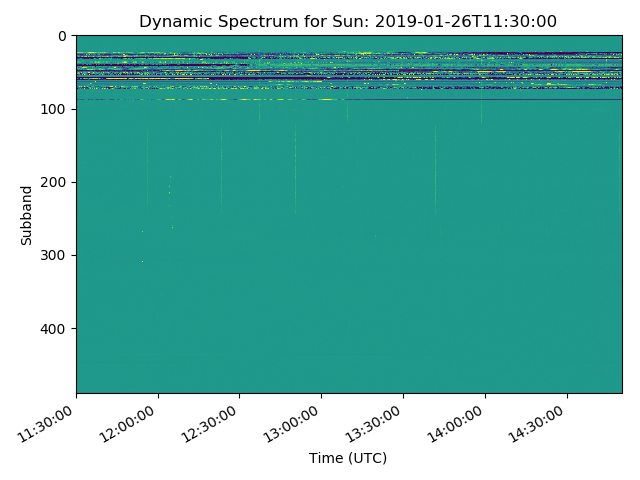
\includegraphics[width=0.5\columnwidth]{Images/Sun_dspec.png}
    \caption[Dynamic spectrum of the Sun on January 29th 2019.]{Dynamic spectrum of the Sun on January 29th 2019 from an observation made with REALTA. The time resolution here has been averaged to 8.1 ms in order to showt the full duration of the observation. A solar flare occurred at 13:21 UTC however no radio activity was detected. The intense bands below subband 100 are due to radio frequency interference (RFI) from short wave radio. Faint vertical lines can be seen between subband 122 and 244 and indicate that a number of packets have been lost between the 4 RSP lanes.}
    \label{fig:blank_dspec}
\end{figure}

\subsection{The TBB Acquisition Cluster (TACl)}
\label{sec:TACl}
TACl is a 6 node computer cluster dedicated to the recording and storage of I-LOFAR TBB data. TACl consists of 4 Dell PowerEdge SC1425 servers, an Isilon IQ 9000X storage server and an Isilon IQ 36NL storage server.
TBB data is recorded to TACl solely by the Isilon IQ 9000X storage server. This is configured in RAID6 in order to write incoming UDP packets containing TBB data to disk. This storage server has 12 disk slots, 8 of which contain Hard Disk Drives (HDDs) that write and store the incoming TBB data at $\sim$ 300MB/s. The remaining 4 slots house 2 disks containing the operating system and 2 Solid State Drives (SSDs) which are being tested as replacements for the HDDs due to their faster data writing speed. The main hurdle in recording TBB data is the disk write speed of TACl. The current solution is to delay each packet so that the previous one can be written to disk. Unfortunately, this increases the amount of time to record on full TBB dump by a great deal, something we hope to overcome by updating the HDDs to faster SSDs.

The Isilon IQ 36NL storage server is intended as general purpose for both TACl and REALTA. Currently most of this storage server is empty containing only one 1 TB HDD and 2 OS disks. Due to the fact that Ubuntu OS and mdraid do not limit storage size, the total possible storage capacity for the Isilon IQ 36NL storage server is  $34 \times 1,2,4,8,16...$TB. 

The Dell PowerEdge SC1425 servers are currently unused but are intended for light data post-processing or could possibly act as a buffer for incoming TBB data using a similar idea to LOFAR's best effort buffer.

Detailed hardware specifications of each server in TACl are shown in Table \ref{table:TAClspecs}.

\begin{center}
\begin{table}[ht]
\centering
\caption[Table of hardware specifications for TACl]{Table of hardware specifications for TACl}
\begin{tabular}{l|l|l}

 & Isilon IQ 9000X & Isilon IQ 36NL \\
\hline
CPU       &  Intel Xeon E5335        & Intel Xeon E5410            \\
CPU Clock Speed & 2.00GHz & 2.33GHz  \\
No. CPU Cores & 4 & 4  \\
RAM       & 1GB          & 4GB            \\
Storage   & 48TB          & 1TB           
\end{tabular}

\label{table:TAClspecs}
\end{table}

\end{center}

It must be acknowledged that without the tireless work of Joe McCauley neither TACl or REALTA would be in their current operational state and recording data from I-LOFAR would be limited to 1 second resolution ``beamlet statistics files".

\subsection{TBB Data Analysis}
\label{sec:tbb_data}
Data recorded using the TBBs are the real voltages induced in the antennas due to radio electromagnetic radiation. The simplicity of this data type makes it incredibly versatile and allows for a ``DIY radio telescope" approach to data analysis. This means that, because TBBs only record voltages at the antenna level they are sensitive to the entire sky. This in turn, means that beamforming can be done in any direction \textit{after} an observation has been made. Beamforming in all directions simultaneously implies imaging in all directions too but this is a much more computationally intensive task. A dedicated high performance computing cluster would be required to maximize the science output of all TBB data recorded. In its current form TACl is mostly useful for recording data only with REALTA doing the bulk of any processing work. Soon, however, REALTA will become dedicated to RSP data and the infrastructure of TACl will have to be improved.

Like RSP data, TBB data is sent from I-LOFAR using UDP packets. This is written to disk with the TBB datawriter described by \cite{Veen2015} in the form of hdf5 format files. This stores both header information and data in a standardised file format making it easily accessible.

First results from analysing TBB data and the analysis software used are described in section \ref{sec:tbb_results} along with a discussion on why further analysis of TBB data has been postponed. 

%Initial efforts in analysing TBB data are described in section \ref{sec:tbb_results} along with a discussion on the temporary discontinuation of this process.
%Initial work in this PhD was centred around obtaining the highest temporal resolution observations of the Sun to date. The task was to use I-LOFAR's TBBs to constantly monitor the Sun and to output when something of interest occurred. Unfortunately, this task requires a lot of technical knowledge and an adequate computer and network set-up, neither of which were present. Regardless, software to beamform data from TBBs was developed and a TBB correlator was utilised to produce prototype dynamic spectra and all-sky images.

%\subsection{Motivation for Study}%(This is why they matter/ what you should have learned)}
%Type III radio bursts are a prevalent feature of radio emission from the Sun. They can occur individually or occasionally in the form of Type III storms which consist of continuous Type III bursts that can last up to days. The defining characteristic of Type III bursts can be recognised in dynamic spectra as a rapid frequency drift from high to low frequencies (see Figure \ref{fig:bursts}). In the case of Type IIIb bursts there exists a fragmented substructure. Other variations of Type III bursts include reverse or bidirectional bursts, which have a positive frequency drift, and U and J bursts, which both show a turning point in frequency drift.

%Type III bursts are caused by electron beams travelling through a slower background of plasma leading to a bump-on-tail instability in the plasma. This means that a positive gradient in the velocity distribution is formed, leading to an instability that causes a rapid growth in the magnitude of Langmuir waves (see Eq. \ref{eq:dWdt}. These Langmuir waves then undergo decay or coalesce with ion sound waves or backward propagating Langmuir waves to produce radio emission at the plasma frequency and its second harmonic respectively. The instability in Langmuir waves is resolved by a diffusive term in Eq. \ref{eq:dfdt} that broadens the bump-on-tail to a plateau, eliminating the positive gradient.

%The study of radio emission from the Sun, Type III bursts in particular, is just as active now as it was immediately after WW2. New instruments like LOFAR and MWA are being used in various ways to observe and study Type III bursts and their sub-categories \citep{Morosan2014,Reid2017ImagingLOFAR, McCauley2017}. The study of Type III bursts give us an insight into the magnetic reconnection that takes place during solar flares. This has implications in space weather research which can have widespread effects here on Earth.

%With new discoveries being made on a regular basis, long disputed questions are being answered and new questions are being asked. The development of the next generation of radio interferometers, the Square Kilometre Array (SKA), will hopefully bring about a new world of information on Type III bursts and the plasma processes that generate them.
%\subsection{Solar Transient Features}
%One of the goals of this PhD is to use REALTA and TACl to observe a number of solar transient features at the highest resolution to date. Current progress on TACl has been slow due to technical problems in TBB data capture and REALTA is operational in a minimal sense however, both show enormous potential for the future. Recent publications on Sbursts, TypeIIIbs and many more show that there is much to be learned if we just had the resolution!

\section{Observing High Spatial Resolution}
\label{sec:event}
The second aspect of this PhD is to study high spatial resolution observations of a solar radio burst. One of the fundamental questions about solar radio observations is: are source sizes what they are observed to be or does scattering in the corona have a major effect? Interferometric observations from LOFAR are one of the best methods of testing this hypothesis, especially if the remote and international stations can be used to generate the longest baselines resulting in sub-arcminute and even sub-arcsecond resolution.

In order to learn more about fine structural scale in the corona and the degree to which scattering affects radio emission, an interferometric dataset of a Type III radio burst is being analysed. The data is taken from 2015-10-17 using all of the core LOFAR stations and 12 of the remote stations, a total of 36 stations, yielding 630 baselines with a maximum of 84 km.
The Type III burst which occurred at 13:21 UTC is briefly described in appendix \ref{app:event}. A spectrum of the Sun was recorded using the LOFAR remote station RS509 from 2015-10-17 08:00 UTC to 2015-10-17 14:00 UTC. The Type III burst is observed in this spectrum at approximately 13:21 UTC as shown in Figure \ref{fig:LOFAR_spec}. Figure \ref{fig:LOFAR_spec} shows the variability in emission of the burst. It is immediately obvious that the Type III burst shows striations, the implications of this will be discussed below.
\begin{figure}
    \centering
    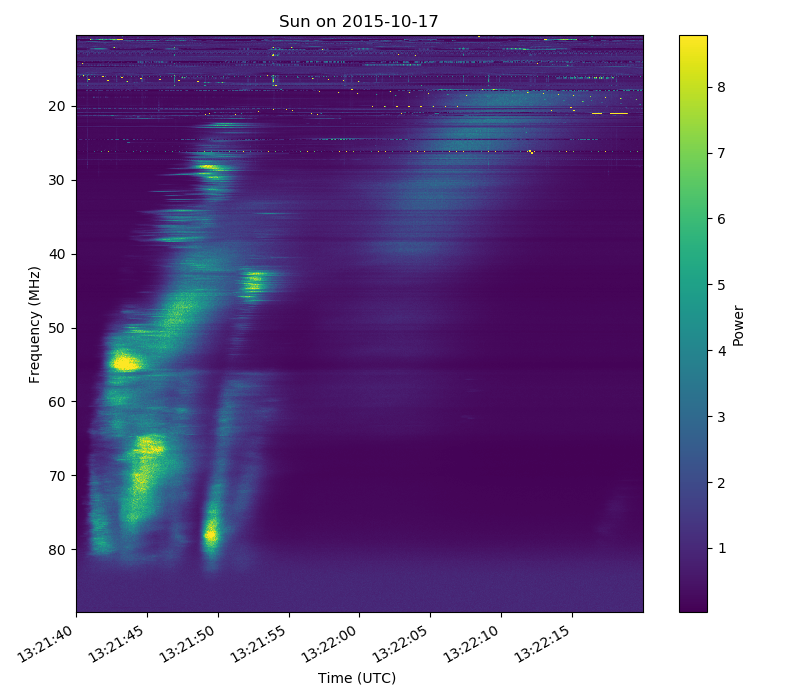
\includegraphics[width=0.75\columnwidth]{Images/L401005_SAP000_B000_S0_P000_bf_d_spec_burst_zoom.png}
    \caption[Type III radio burst observed with LOFAR station RS509]{a) Type III radio burst observed with LOFAR station RS509 in the north of the Netherlands. A plethora of temporal and frequency variation can be seen over the burst's duration.}
    \label{fig:LOFAR_spec}
\end{figure}
% The Type III burst which occurred at 13:21 UTC is shown in the composite radio spectra in Figure \ref{fig:comp_spec} and was not co-temporal with any other solar event.

% \begin{figure}
%     \centering
%     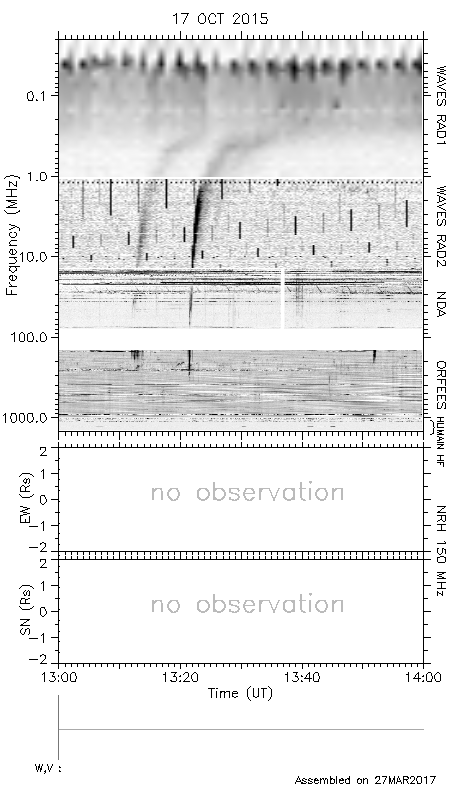
\includegraphics[width=0.75\columnwidth]{Images/Radio_composite.png}
%     \caption[Composite of radio spectra from multiple ground and space based radio telescopes.]{Composite of radio spectra from multiple ground and space based radio telescopes. From top to bottom these include; WAVES RAD1, WAVES RAD2 (both on board the WIND space craft), the Nan\c{c}ay Decametric Array (NDA), ORFEES radio-spectrograph (Observations Radio pour Fedome et l’Etude des Eruptions Solaires) and the Nan\c{c}ay Radio Heliograph (NRH, no data). A Type III radio burst is seen as a dark streak after 13:20 in all 4 spectra.}
%     \label{fig:comp_spec}
% \end{figure}

% EUV images of the Sun such as those taken in the 193{\AA} channel with AIA, Figure \ref{fig:AIA_GOES}a, show a number of bright active regions and a coronal hole which give indications of where to expect closed and open magnetic field lines.
% Xray flux around the time of the Type III burst was measured by the Geostationary Operational Environmental Satellite (GOES, seen in Figure \ref{fig:AIA_GOES}b). It should be noted that there were a number of small C class solar flares before the radio burst however none were co-temporal. 


% \begin{figure}
%     \centering
%     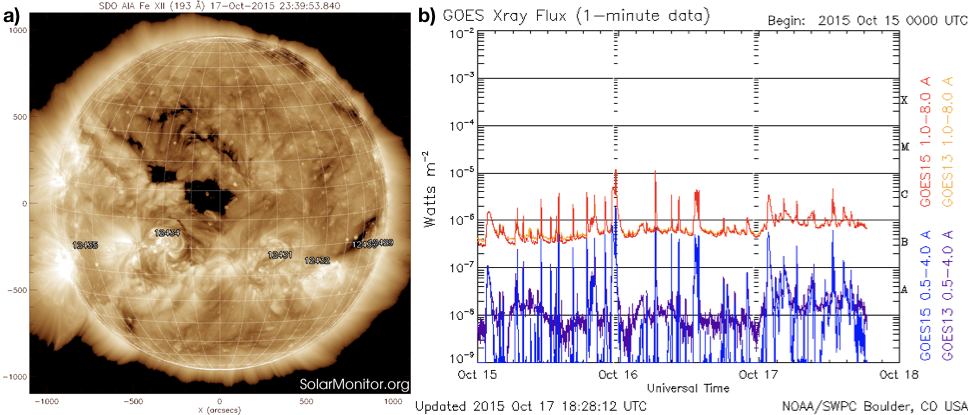
\includegraphics[width=\columnwidth]{Images/aia_goes.png}
%     \caption[193 {\AA} image of the Sun taken by AIA and Xray flux as measured by GOES on 2015-10-17]{a) 193 {\AA} image of the Sun taken by AIA on 2015-10-17 b) Xray flux as measured by GOES on 2015-10-17.}
%     \label{fig:AIA_GOES}
% \end{figure}


% % \begin{figure}
% %     \centering
% %     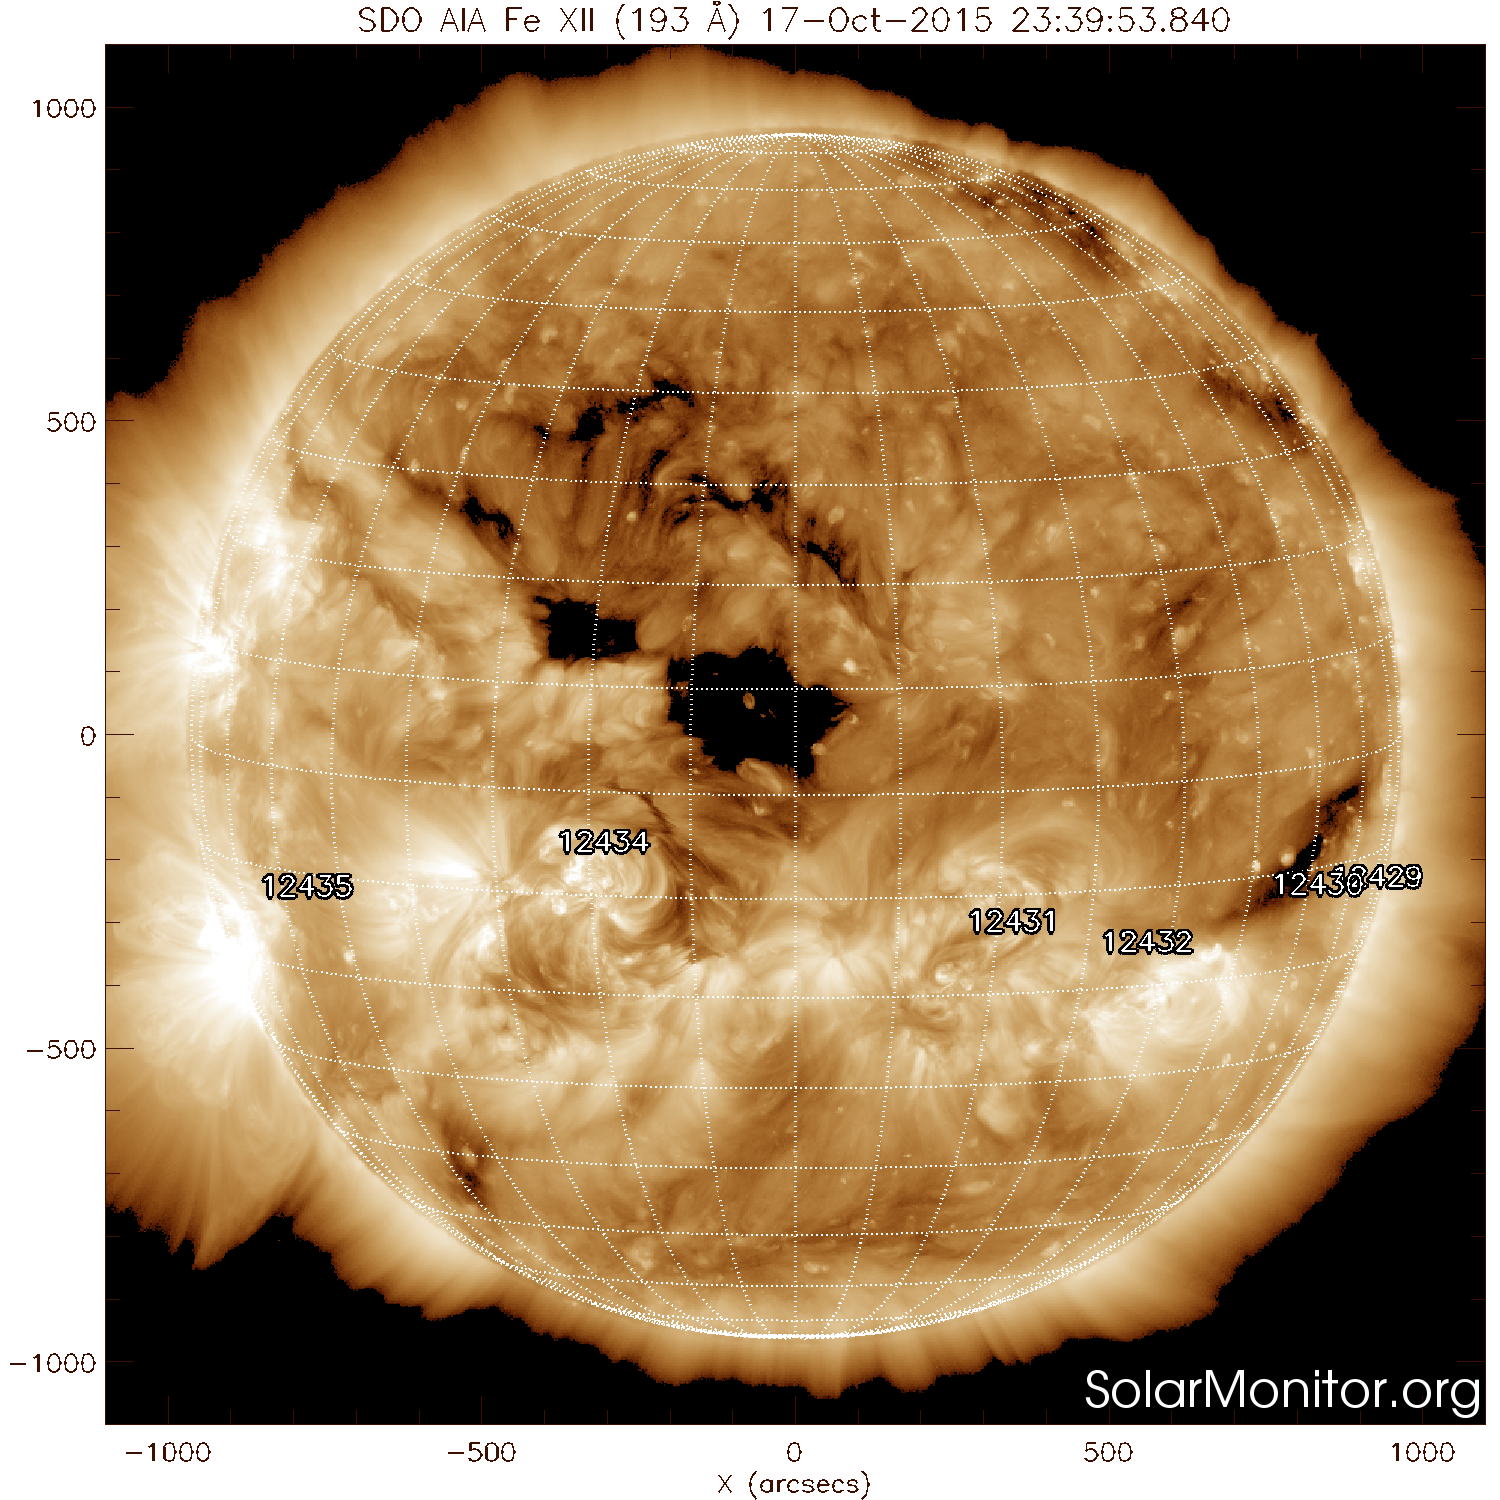
\includegraphics[width=0.75\columnwidth]{Images/aia_193.png}
% %     \caption[193 {\AA} image of the Sun taken by AIA on 2015-10-17]{193 {\AA} image of the Sun taken by AIA on 2015-10-17}
% %     \label{fig:aia193}
% % \end{figure}

% A spectrum of the Sun was recorded using the LOFAR remote station RS509 from 2015-10-17 08:00 UTC to 2015-10-17 14:00 UTC. The Type III burst is observed in this spectrum approximately 19300s after the observation start as shown in Figure \ref{fig:LOFAR_spec}a. Figure \ref{fig:LOFAR_spec}b shows the burst over a shorter time scale thus allowing the variability in emission to be seen.
% \begin{figure}
%     \centering
%     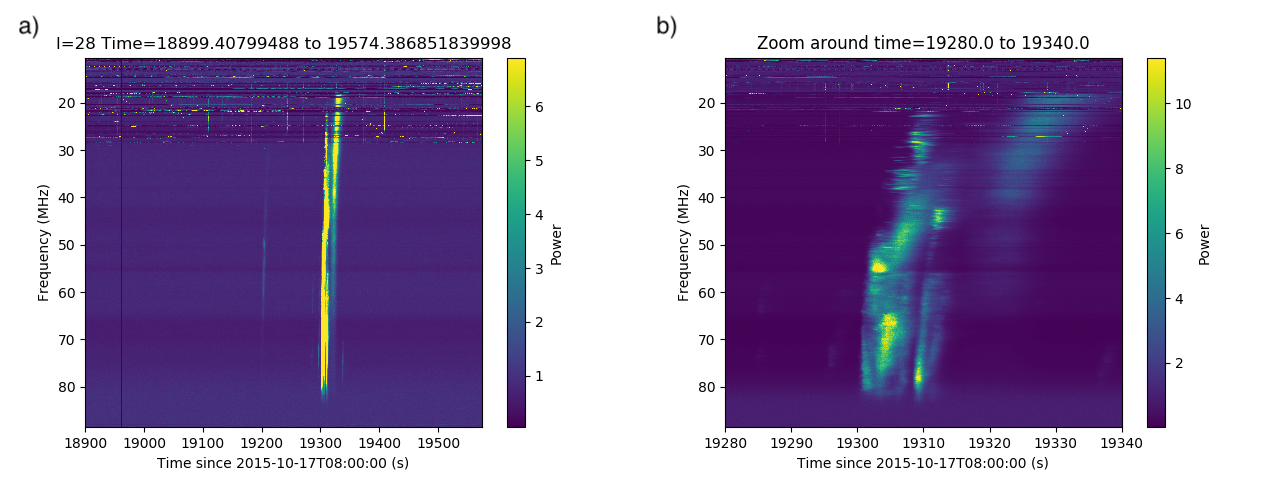
\includegraphics[width=\columnwidth]{Images/L401005_SAP000_B000_S0_P000_bf_d_spec_composite.png}
%     \caption[Type III radio burst observed with LOFAR station RS509]{a) Type III radio burst observed with LOFAR station RS509 in the north of the Netherlands. b) A zoom in of the Type III burst, a  plethora of temporal and frequency variation can be seen over the burst's duration.}
%     \label{fig:LOFAR_spec}
% \end{figure}

The most common observational method for Type III bursts with LOFAR is the tied-array imaging mode \citep{Morosan2014} whereby a number of LOFAR ``station beams", formed by combining all the antennas in a single LOFAR station, are added coherently to create tied-array beams. These beams are then tessellated across the Sun and an image reconstructed from the spectra of each beam. This imaging mode has the benefit that it retains the 5.12 $\mu$s resolution but accurately determining source size and position becomes an issue due to multiple beams detecting radio emission. Interferometric imaging therefore gives a more accurate spatial resolution of a burst at the cost of one image every 0.25 s.


%\chapter{Results \& Interpretation}
%\label{chap:results}
%Results from TBB observations are described here along with preliminary images of a Type III burst. 

\section{TBB Results}
\label{sec:tbb_results}
The initial work during this PhD was done on building a data analysis pipeline for TBB data from I-LOFAR. At the time, TACl (section \ref{sec:TACl}) was still in its early stages of operation and testing of data acquisition method indicated much more needed to be done to capture TBB data at a sufficient rate. Despite this, a moderate codebase (\url{https://github.com/ILOFAR/TBB_scripts}, described below) was created in order to analyse this ``commissioning data". This software allows TBB data to be beamformed in any direction on the sky to produce a dynamic spectrum such as the prototype dynamic spectrum of the Sun in Figure \ref{fig:proto_dspec}. These dynamic spectra can cover any frequency range within the observed band with the limiting factor on frequency resolution being computer power and the size of the Fourier window. Section \ref{sec:TBB_software} describes how the software written in the first few months of this PhD produced the highest temporal resolution observations ever achieved.
\begin{figure}
    \centering
    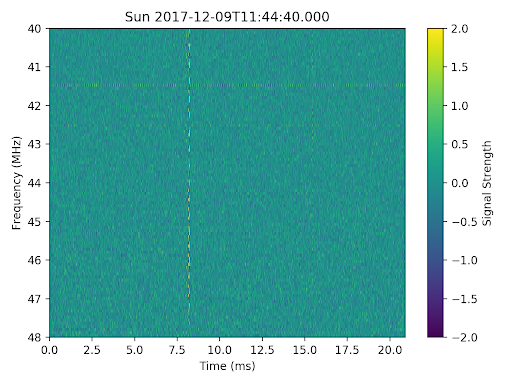
\includegraphics[width=0.5\columnwidth]{Images/TBB_dspec.png}
    \caption[Prototype TBB dynamic spectrum]{A prototype TBB dynamic spectrum created using code written in the first few months of this PhD.}
    \label{fig:proto_dspec}
\end{figure}


A correlator for TBB data (\url{https://github.com/sabourke/tbb-correlator}) was utilised to produce the prototype all sky image of Figure \ref{fig:proto_allsky}a. In order to correlate data correctly, all input data must have the exact same start time. This criterion was only fulfilled by 7 antennas leading to poor a \textit{uv} coverage. Figure \ref{fig:proto_allsky}b shows the point spread function (PSF) of the 7 element array which is shown to have several bright spots in a pattern around the main beam, these are the sidelobes of the antenna beam.
\begin{figure}
    \centering
    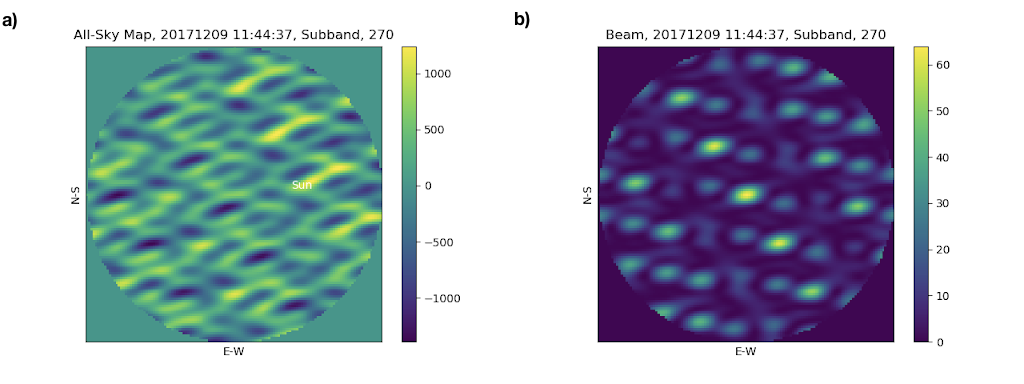
\includegraphics[width=\columnwidth]{Images/AllSky_psf.png}
    \caption[Prototype TBB all sky image]{a) A prototype all sky image made from TBB data. Technical difficulties in recording data with a precise start time meant that only data from 7 antennae could be correlated to produce this image. This resulted in the point spread function b) containing numerous sidelobes. }
    \label{fig:proto_allsky}
\end{figure}

Despite the potential of TBB data to revolutionise solar observations, difficulties in acquiring it reliably mean that development of this code and analysis of TBB data are to be postponed until analysis of an interferometric observation of a Type III burst (section \ref{sec:event}) is complete.
% beam with numerous sidelobes, this in turn produced the low quality image shown.
\subsection{TBB Software}
\label{sec:TBB_software}
In order to create dynamic spectra from TBB data, the channelisation of a LOFAR RSP board must be replicated. For brevity's sake, the following discussion will ignore the procedure to beamform as it is simply an implementation of the theory described in section \ref{sec:beamform_theory}. 

In order to preserve the 5 ns time resolution of TBB data the raw voltage data must first undergo a Fourier transform. This can be though of as representing the entire signal time series as power per frequency with frequency resolution governed by the relation from a discrete Fourier transform (DFT),
$$\Delta f = \frac{1}{N\Delta t}$$
where $\Delta f$ is the frequency resolution, $N$ is the number of points the DFT uses and $\Delta t$ is the time resolution. Depending on the desired frequency resolution, the data spectrum obtained from the DFT is then split into a number of ``subbands" which are analogous to subbands produced in an RSP board (Figure \ref{fig:subbands_pspec}a). One subband is selected while the rest of the spectrum is set to zero so that an inverse DFT can be performed resulting in the initial 5 ns time resolution. This is done for each subband so that a number of time series at a particular frequency range are created. These time series are then stacked and represented as a dynamic spectrum such as the one in Figure \ref{fig:subbands_pspec}b.

\begin{figure}
    \centering
    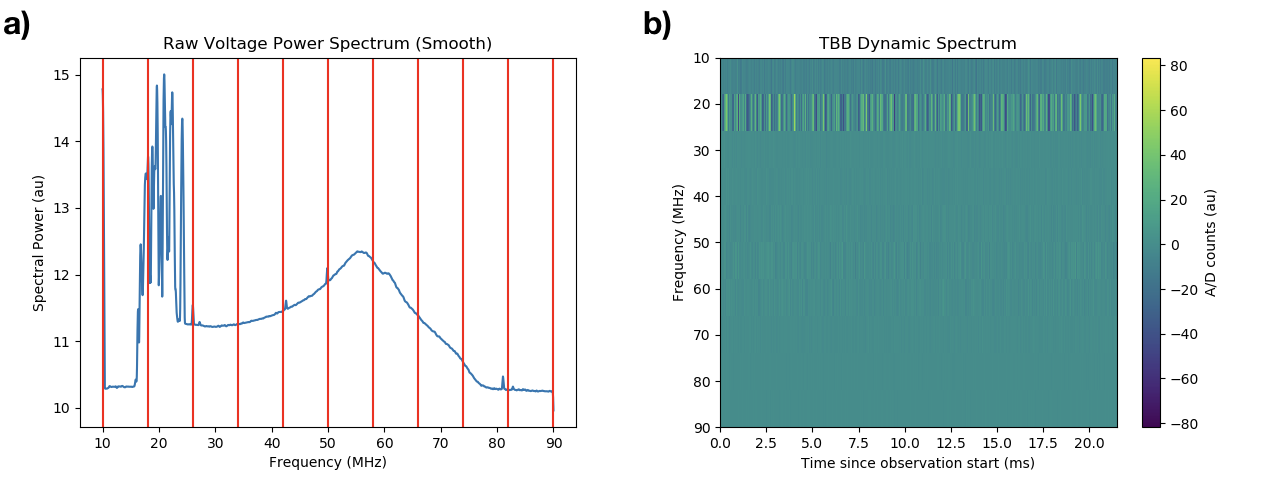
\includegraphics[width=\columnwidth]{Images/TBB_spectra.png}
    \caption[Spectrum of TBB data and subbands]{a) A sample spectrum of TBB data. The spectrum is smoothed for clarity and the subband edges are shown as red vertical lines. b) The dynamic spectrum by channelising in the method outlined above.}
    \label{fig:subbands_pspec}
\end{figure}

% \begin{figure}[t]
%     \centering
%     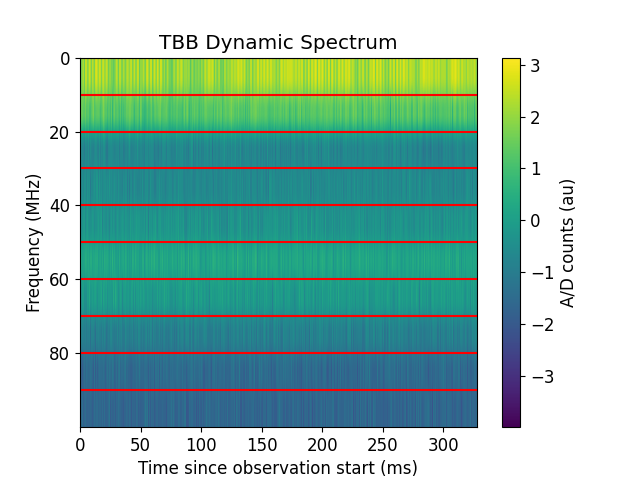
\includegraphics[width=0.75\columnwidth]{Images/TBB_dynamic_spectrum.png}
%     \caption[Dynamic spectrum of TBB data]{The dynamic spectrum by channelising in the method outlined above.}
%     \label{fig:TBB_dspec}
% \end{figure}

Performing channelisation in this way gives a user the freedom to select any frequency range to channelise within the band with any frequency resolution. There are however, a few undesired effects of too fine a frequency resolution. Firstly, windowing a DFT produces unwanted sidelobes in the reconstructed time series and also serves to broaden sharp peaks. Before further work can be done using this code, the effects of different DFT window sizes must be characterised.

Once TACl can record TBB data reliably, development and implementation of the existing code can continue. It is hoped that by the end of this PhD that ``quick look" plots of TBB data can be produced in almost real time as the data is being recorded in order to automatically discern whether there is an event of interest or if the data can be deleted. It is expected that a number of machine learning algorithms will be utilised in this process.

\section{Interferometric Results}
Figure \ref{fig:typeIIIcomp} shows a number of preliminary interferometric images at different wavelengths of the Type III burst described in appendix \ref{app:event}. Here, 4 subbands corresponding to 29.68 MHz, 39.45 MHz, 49.21 MHz and 63.28 MHz of the burst are displayed at the time 13:21:55.6. The red crosses in each panel indicate the centre of the Sun and the point of maximum intensity in the burst, the red circle shows the size of the Sun.
This type of interferometric observation gives a great opportunity to study Type III emission from the perspective of both burst dynamics and radio wave propagation. Positional tracking of a Type III burst was carried out by \cite{Mann2018} and is the only study of its kind. However, the dynamic spectra were reconstructed from the images and not recorded in LOFAR beam-formed mode, as is the case for this observation. % Thus, more detailed spectral and temporal characteristics than the be studied.
Type III bursts are sometimes observed to contain fine spectral structures known as striae. These can be used to give an order of magnitude limit to the source size of density inhomogoneities in the solar corona as was described in \cite{Kontar2017}. 
The Type III burst captured in this data also contains striae (Figure \ref{fig:LOFAR_spec}) meaning a direct comparison with \cite{Kontar2017} can be made. Controversy exists as to whether the conclusions from \cite{Kontar2017} are a result of coronal scattering, as claimed, or are due to the extended beam size of tied-array imaging. Analysis of the event described above will be a further piece of evidence in support of/against the importance of coronal scattering.

%thus clearing some controversy in the solar community as it will be the first time this study is done using interferometric imaging instead of tied-array imaging.

From the preliminary images in Figure \ref{fig:typeIIIcomp} it is immediately obvious that the source sizes in these images are smaller by a large amount than suggested by \cite{Kontar2017} who present source sizes of the order 20 arcminutes. %The Type III source can be seen at a greater distance from the Sun with decreasing frequency as expected from the plasma emission theory of Type III bursts, which suggests that lower frequencies correspond to lower electron densities and thus, greater heights in the solar corona.
\begin{figure}[t]
    \centering
    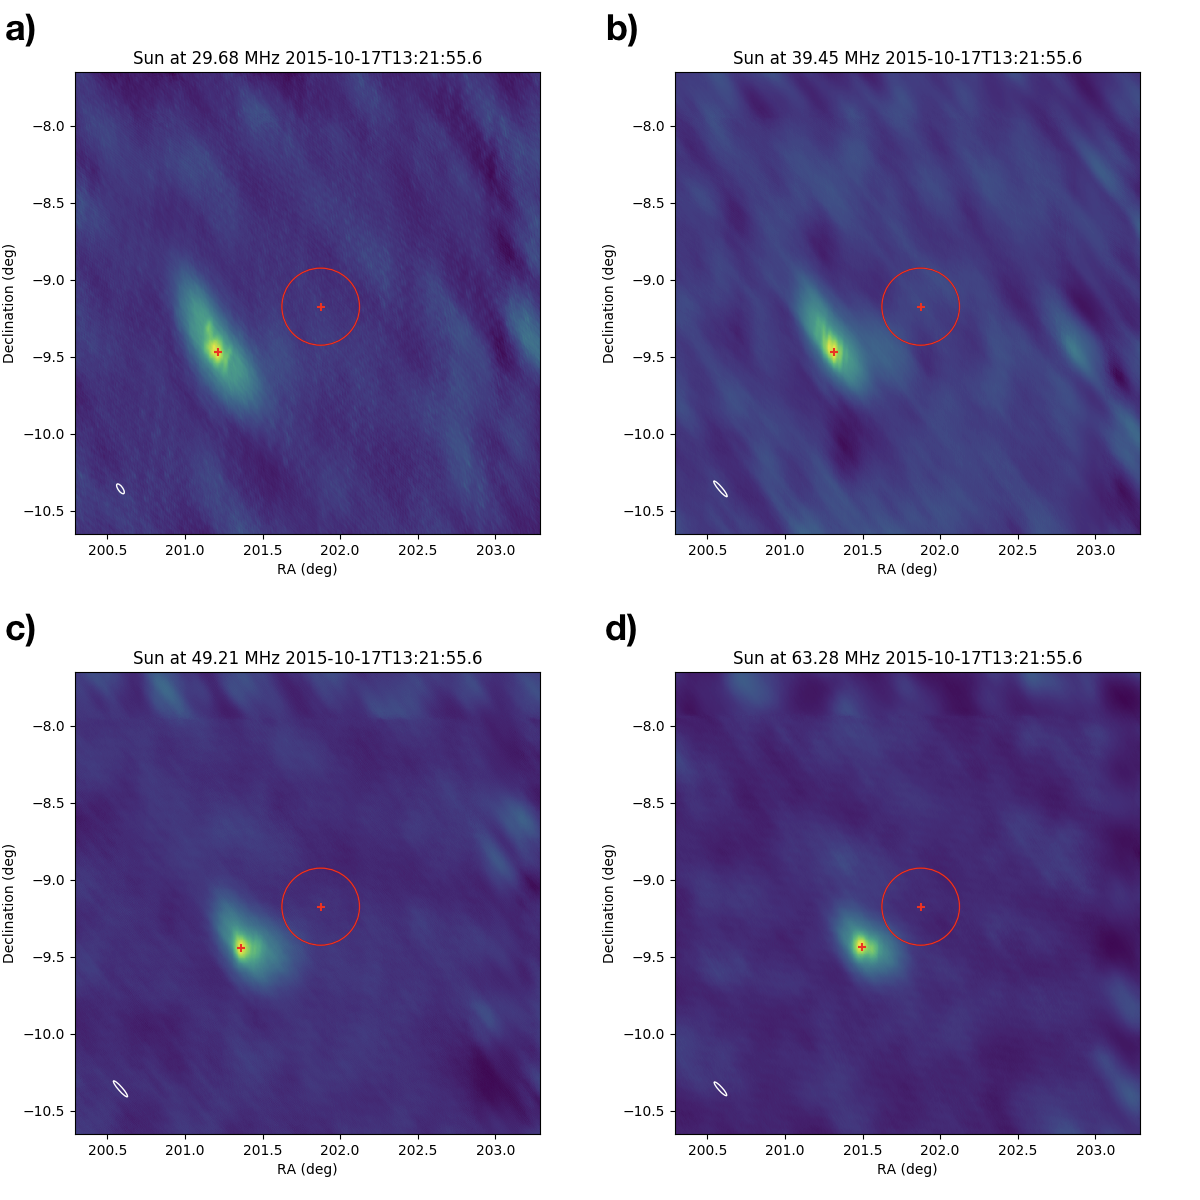
\includegraphics[width=0.75\columnwidth]{Images/TypeIII_comparison.png}
    \caption[Interferometric images of a Type III burst]{Interferometric images of a Type III burst at 13:21:55.6 on 2015-10-17 at 4 different frequencies a) 29.68 MHz b) 39.45 MHz c) 49.21 MHz d) 63.28 MHz. The red circle in each panel indicates the size of the Sun and the two red crosses indicate the centre position of the Sun and the position of maximum intensity in each panel. The with ellipse indicates the shape and position of the LOFAR beam.}
    \label{fig:typeIIIcomp}
\end{figure}

The images I have created thus far have yet to undergo a thorough analysis of the effects of parameters used in the WSCLEAN algorithm \citep{Offringa2014}, one of the main deconvolutional methods used to produce interferometric images. Different weighting schemes prioritise different spatial scales in interferometric observations. Knowing that coronal scattering may effect observed source sizes, extreme care must be taken before any conclusive inferences are drawn from images produced. An initial inspection of Figure \ref{fig:typeIIIcomp} suggests the source size of the Type III burst to be of the order of the size of 0.5 R$_{\odot}$ at lower frequencies and $\sim 1 \mbox{ R}_\odot$ at higher frequencies. 











%%!TEX root = ../main.tex
%Adding the above line, with the name of your base .tex file (in this case "thesis.tex") will allow you to compile the whole thesis even when working inside one of the chapter tex files
%%
%%
\onehalfspacing
\chapter{Conclusion}
\label{chap:conc}
The solar corona produces a number of radio phenomena, some of which well understood and others less so. The resolution at which the Sun can be observed in metric wavelengths has increased dramatically over the last 20 years both spatially and temporally. Current generation radio interferometers such as LOFAR offer sub-arcminute spatial resolution when imaging and can produce spectra with a temporal resolution of 5.12 $\mu$s. 

The use of I-LOFAR in single station mode allows us access to an additional data recording source, the Transient Buffer Boards (TBBs) which can store raw voltage data at a temporal resolution of 5 ns. I have writeen software to not only create spectra from this data but also to ``point" I-LOFAR at a position on the sky in post-processing. This allows, for the first time, the corona to be studied at the nanosecond timescale and turns I-LOFAR to one of the world's most powerful solar spectrometers. 

Two computer clusters located in the I-LOFAR control room at the Rosse Observatory, Birr, Co. Offaly, record and analyse data from I-LOFAR's Remote Station Processing boards (RSPs) and TBBs. These are the REALtime Transient Acquisition cluster (REALTA) and the TBB Acquistion Cluster (TACl). Both REALTA and TACl have been set up to be in their current operational state and are able to record data at an acceptable rate. Additional work is being undertaken to parallelise recording and data analysis to vastly increase the scientific output from both clusters. Collaboration with Griffin Foster of the Breakthrough Foundation to improve REALTA so that it can perform operations on data as it is being recorded is ongoing while colaboration with Dr. Brian Coghlan from the School of Computer Science and Statistics regarding TACl also continues.

Interferometric data obtained from the LOFAR core and remote stations on 2015-10-17 from 08:00 UTC to 14:00 UTC is currently being analysed. During this time, at 13:21 UTC, a Type III burst occurred and can be seen in LOFAR beamformed observations (Figure \ref{fig:LOFAR_spec}). Preliminary images of this burst have been made using the WSCLEAN algorithm (Figure \ref{fig:typeIIIcomp}) with an appropriate weighting scheme to be decided upon. The Type III burst shows striations in its spectrum making a direct comparison between the work of \cite{Kontar2017} using interferometric imaging rather than tied-array imaging possible. Regardless of whether this work agrees or disagrees with \cite{Kontar2017}, the result will have significant implications for radio solar physics and will either prove that there is a fundamental resolution beyond which we cannot see or, the limit does not exist and interferometric observations with longer baselines will open up further study into the solar corona for years to come. %It is hoped that this analysis will find the extent to which scattering from density inhomogeneities in the corona has on the observed source sizes at metric wavelengths.








%%!TEX root = ../main.tex
%Adding the above line, with the name of your base .tex file (in this case "thesis.tex") will allow you to compile the whole thesis even when working inside one of the chapter tex files
%%
%%
%%%%%%%%%%%%%%%%%%%%%%%%%%%%%%%%%%%%%%%%%%%%%%%%%%%%%%%%%%%%%%%%%%%%%%%%%%%%%
%%%%%%%%%%%%%%%%%%%%%%%%%%%%%%%%%%%%%%%%%%%%%%%%%%%%%%%%%%%%%%%%%%%%%%%%%%%%%
%%%%%%%%%%%%%%%%%%%%%%%%%%%%%%%%%%%%%%%%%%%%%%%%%%%%%%%%%%%%%%%%%%%%%%%%%%%%%
%										FUTURE WORK
%%%%%%%%%%%%%%%%%%%%%%%%%%%%%%%%%%%%%%%%%%%%%%%%%%%%%%%%%%%%%%%%%%%%%%%%%%%%%
%%%%%%%%%%%%%%%%%%%%%%%%%%%%%%%%%%%%%%%%%%%%%%%%%%%%%%%%%%%%%%%%%%%%%%%%%%%%%
%%%%%%%%%%%%%%%%%%%%%%%%%%%%%%%%%%%%%%%%%%%%%%%%%%%%%%%%%%%%%%%%%%%%%%%%%%%%%
\onehalfspacing
\chapter{Future Work}
\label{chap:future}
%The future work of this PhD will be twofold combining the technical tasks required to get REALTA and TACl working to their full potential, 
The future work of this PhD can be divided into 3 main topics; technical work with REALTA and TACl, analysis of fine spatial structure in a complex radio burst, and radio frequency interference (RFI) removal using machine learning. A Gantt chart for the remainder of this PhD is shown in Figure \ref{fig:Gantt}

\begin{figure}[t]
    \centering
    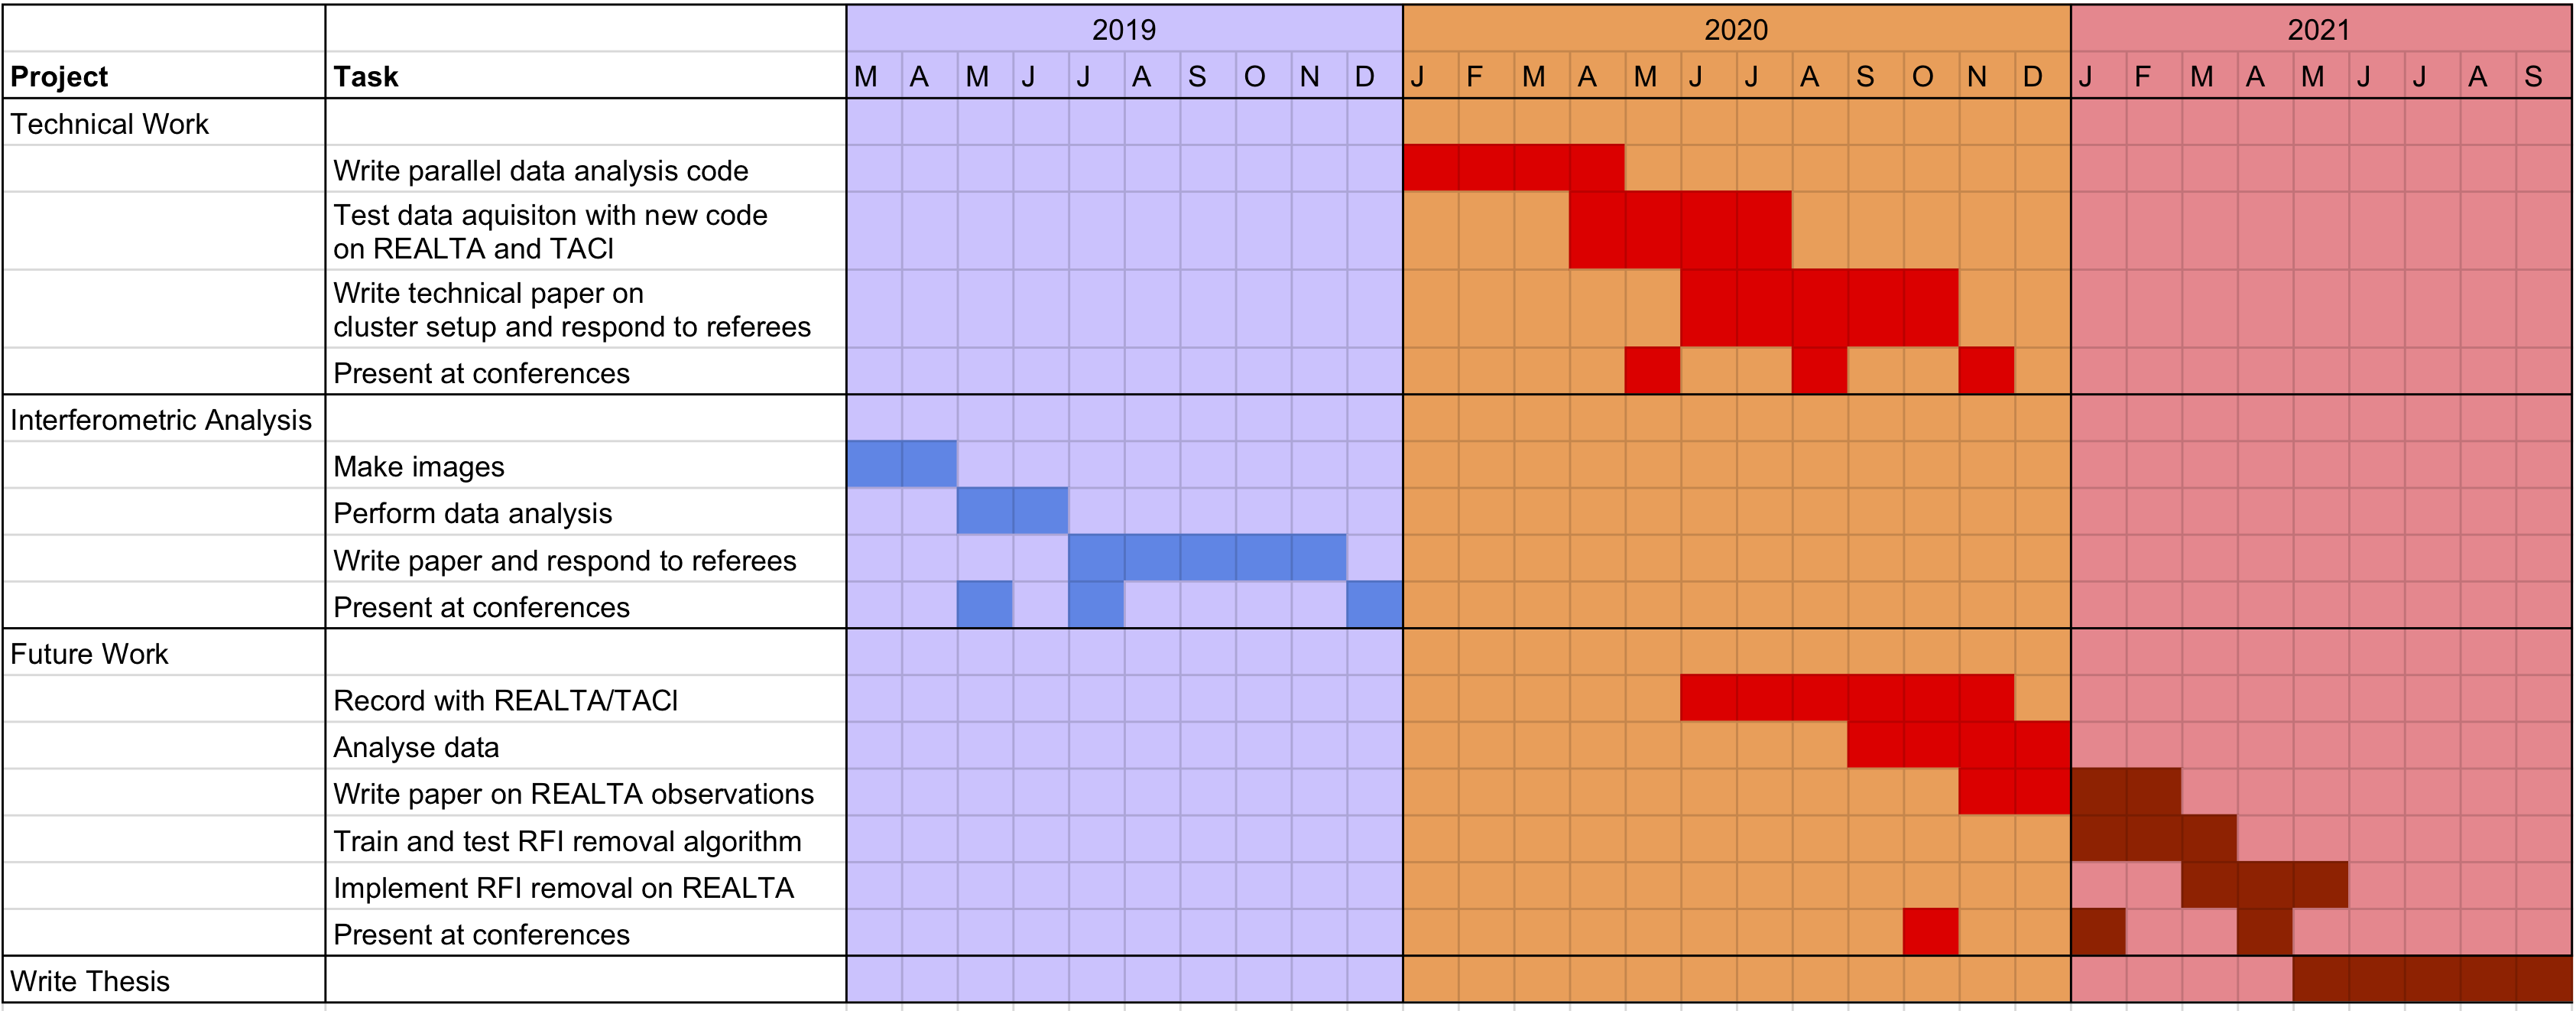
\includegraphics[width=0.75\columnwidth]{Images/PM_Ganttchart.png}
    \caption[Gantt chart for remainder of PhD]{Gantt chart for remainder of PhD}
    \label{fig:Gantt}
\end{figure}

\section{Technical Work}
Both REALTA and TACl are operational in a minimal sense although there is still work to be done in order to develop them to become bona fide telescope backends. Data recorded by TACl in the last number of months has been partially corrupted and the cause is still being investigated with Dr. Brian Coghlan of the School of Computer Science and Statistics. Once operational, TACl will be able to record TBB data again and the development of software to analyse this data will be continued. Despite being in solar minimum, approximately 2,355 radio bursts are expected to occur per year \citep{Nita2002}. This give ample opportunity to detect a radio burst and study it at the highest temporal resolution ever. %It is expected that some sort of solar radio phenomenon will be detected by the TBBs and analysed before the end of this PhD.

REALTA also requires further setup before it can be used as a parallel GPU-based cluster. A head node to control the cluster operations was installed in November 2018 and collaboration with Griffin Foster (Oxford, Berkeley, Breakthrough) will continue in order to write GPU-based code for data capture and analysis. This will make observations of the Sun more accessible than they are currently which should result in greater scientific output.

After REALTA is capable of performing analysis on incoming data in real time a paper discussing the hardware and software setup required to do so could be written. This would be the first of its kind for an international LOFAR station and would hopefully inspire other international station owners to improve their own computing hardware. This would allow the possibility of more computationally intense collaborations with other international stations operating in single station mode.

\section{Interferometric Analysis}
Analysis of the burst event described in section \ref{sec:event} will continue and be presented at an international conference by the end of 2019. It is expected that this analysis will put a limit on how much scattering affects radio propagation in the corona. If it is shown that there is no fundamental limit to spatial resolution at metric limits this will strengthen the case to observe the Sun with the full $\sim 2000$ km international baseline offered by LOFAR.

There are a number of steps that must be carried out before this can be done however, the most immediate of which is to account for the change in coordinate systems from topocentric (from the viewers perspective) to heliocentric (centred on the Sun). This will allow close comparison of radio and other wavelength observations, e.g. EUV data from AIA, as this is the standard coordinate system used in solar physics.
The imaging of this event must also be thoroughly investigated as a change in the parameters used in the WSCLEAN algorithm can result in drastically different images. As such, weighting schemes, number of iterations and more must be considered with great thought before data analysis of images can begin.
Once images have been created, the spatial scale and distance from the centre of the Sun will be measured in order to obtain a measure on how much propagation effects in the corona effect the measurement.

The existence of striae in the Type III spectrum offer a direct comparison with the work by \cite{Kontar2017} using interferometric imaging for the first time. It is expected that this work will be submitted as a letter at a well renowned journal such as the Astrophysical Journal.

\section{RFI Removal}
Radio Frequency Interference often obscures signals of interest in dynamic spectra and usually washes out weaker signals because it is so intense. Great effort is made in the design of radio telescopes to mitigate the effects of nearby electronics however to eliminate all RFI completely would require such a massive societal involvement that it will never happen. Thus, removal of RFI is done after data has been recorded using algorithms developed to identify RFI based on its spectral properties \citep{Offringa2012b, Nita2007}.

Machine learning techniques can be used to detect and remove RFI without the need to define an algorithm based on RFI structure. An approach to removing RFI is inspired by a transient detection system described by \cite{Sedaghat2018}. A convolutional autoencoder (CAE) is a machine learning algorithm using convolutional layers in a traditional autoencoder \citep{Vincent2008}. A CAE would be used to first encode a spectrum containing RFI to a more simple form and then decode to return the spectrum without RFI. This procedure is known as ``denoising" and has seen success in a number of classical machine learning problems. To train the network successfully will require many hundereds of thousands of sample spectra. One hundred thousand LOFAR LBA spectra have been simulated, these will be used as a first attempt training set for the CAE and its performance will be tested on 20\% of these spectra. It is anticipated to test this network on real I-LOFAR data in conjuction with an automatic burst detection network developed by Dr. Eoin Carley of the Solar and Space Weather group.


%Currently this project is in its early stage but is outlined as follows. 100000 LOFAR spectra are simulated with and without RFI. These spectra will be fed into what is known as a convolutional encoder-decoder network or convolutional autoencoder (CAE) which will learn how to remove RFI without the need for a pre-made algorithm based on the physics of RFI, such as spectral kurtosis RFI removal described by \cite{Nita2007}. CAEs are based on the principals of autoencoders described in \cite{Vincent2008} but using the convolutional methods that have seen great success in image processing.


% --------------------------------------------------------------
%:                  BACK MATTER: appendices, refs,..
% --------------------------------------------------------------

%: ----------------------- bibliography ------------------------

\newgeometry{left=1.6cm, right=1.6cm, top=-2.0cm, bottom=1.0cm, footskip=0cm}
\singlespacing
\begin{footnotesize} 
\bibliographystyle{aa}
\renewcommand{\bibname}{References} 
%\begin{multicols}{2}

\bibliography{thesis_references}

%\end{multicols}

\singlespacing
\end{footnotesize}
\restoregeometry

\appendix
%%!TEX root = ../main.tex
%Adding the above line, with the name of your base .tex file (in this case "thesis.tex") will allow you to compile the whole thesis even when working inside one of the chapter tex files

% \chapter{TBB Software}
% \label{app:TBB_software}
% In order to create dynamic spectra from TBB data, the channelisation of a LOFAR RSP board must be replicated. For brevity's sake, the following discussion will ignore the procedure to beamform as it is simply an implementation of the theory described in section \ref{sec:beamform_theory}. 

% In order to preserve the 5 ns time resolution of TBB data the raw voltage data must first undergo a Fourier transform. This can be though of as representing the entire signal time series as power per frequency with frequency resolution governed by the relation from a discrete Fourier transform (DFT),
% $$\Delta f = \frac{1}{N\Delta t}$$
% where $\Delta f$ is the frequency resolution, $N$ is the number of points the DFT uses and $\Delta t$ is the time resolution. Depending on the desired frequency resolution, the data spectrum obtained from the DFT is then split into a number of ``subbands" which are analogous to subbands produced in an RSP board (Figure \ref{fig:subbands_pspec}). One subband is selected while the rest of the spectrum is set to zero so that an inverse DFT can be performed resulting in the initial 5 ns time resolution. This is done for each subband so that a number of time series at a particular frequency range. These time series are then stacked and represented as a dynamic spectrum such as the one in Figure \ref{fig:TBB_dspec}.

% \begin{figure}
%     \centering
%     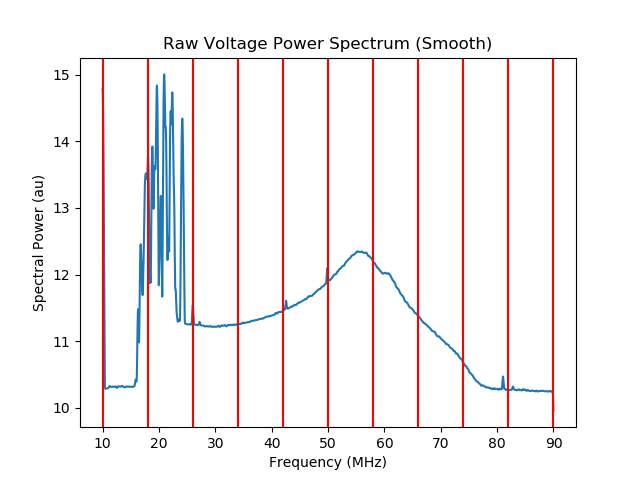
\includegraphics[width=0.75\columnwidth]{Images/p_spec_smooth.png}
%     \caption[Spectrum of TBB data and subbands]{A sample spectrum of TBB data. The spectrum is smoothed for clarity and the subband edges are shown as red vertical lines.}
%     \label{fig:subbands_pspec}
% \end{figure}

% \begin{figure}
%     \centering
%     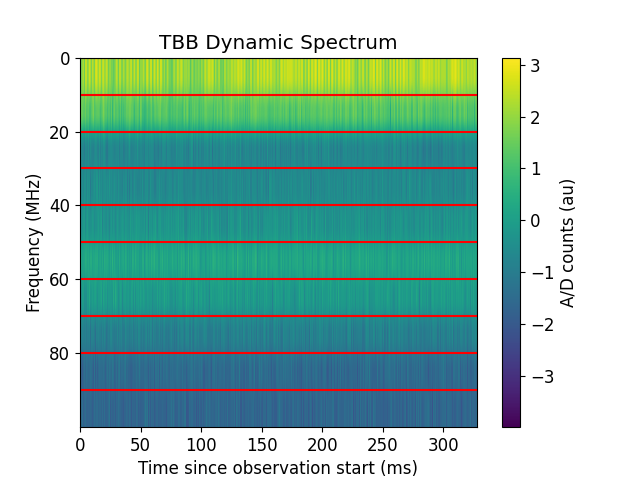
\includegraphics[width=0.75\columnwidth]{Images/TBB_dynamic_spectrum.png}
%     \caption[Dynamic spectrum of TBB data]{The dynamic spectrum by channelising in the method outlined above.}
%     \label{fig:TBB_dspec}
% \end{figure}

% Performing channelisation in this way gives a user the freedom to select any frequency range to channelise within the band with any frequency resolution. There are however, a few undesired effects of too fine a frequency resolution. Firstly, windowing a DFT produces unwanted sidelobes in the reconstructed time series and also serves to broaden sharp peaks. Before further work can be done using this code, the effects of different DFT window sizes must be characterised.
%  %There is one major distinction between the channelisation in an RSP and in software.

\chapter{Plasma Emission}
\label{app:plasma}
In 1942 while Britain was on the look out for radar signals of enemy aircraft, a strong, noise like and highly variable signal was noticed by radar operators. Initially it was thought that Germany had managed to learn the secret of radar and create some sort of jamming device. On further investigation it was found that this jamming was in fact radio emission from the Sun. The discovery of this radio emission being associated with a major solar flare was kept secret until after the war and was published by \cite{Appleton1946}.
Since then a number of major advancements in both instrumentation and theory have occurred. A culmination of the theory of solar radio emission is laid out in the book by \cite{McLean1985} while worldwide, a number of extraordinary radio telescopes and interferometers such as the LOw Frequency ARray (LOFAR, \citeauthor{VanHaarlem2013b} \citeyear{VanHaarlem2013b}), the Nan\c{c}ay Radio Heliograph and the Murchison Widefield Array (MWA), to name but a few, have been built.

Solar radio emission often comes in the form of bursts of varying timescales. These were initially classified into three types by \cite{Wild1950b} with a fourth and fifth type being discovered by \cite{Boischot1957} and \cite{Wild1959} respectively. Of these, the most frequently occurring are the so called Type III radio bursts. These are short bursts that can be observed over many frequencies and are found to be associated with solar flares \citep{Malville1962}. An initial study into how they are emitted was conducted by \cite{Ginzburg1958}.% This essay examines Type III bursts and in particular describes their observed characteristics, what causes them and the plasma emission process of their generation.

%\section{Process of Forming Type III Bursts} %(This is how they're made)}
For a Type III radio burst to be emitted, an electron must generate Langmuir waves in the plasma. These Langmuir waves then go on to generate electromagnetic transverse waves by coalescing with other waves or by decaying. Theses electromagnetic waves are the radio bursts that are observed. In this section the generation of Langmuir waves and the process of plasma emission are discussed.

\section{Generation of Langmuir Waves}
During magnetic reconnection in a solar flare electrons are accelerated along magnetic field lines. As these beams of electrons propagate, faster electrons begin to outpace slower electrons and stationary ions in the background plasma. This leads to a second peak on the Maxwell Boltzmann distribution of velocities as seen in Figure \ref{fig:Lwavegrowth}. Energy is transferred from electrons electrons travelling at the phase velocity, $v_{\phi}$ , to Langmuir waves creating a resonance.
The positive velocity gradient of this resonance means that there are more electrons with velocity greater than $v_{\phi}$ than there are electrons with velocities less than  $v_{\phi}$ (where energy is transferred from the wave to the particles), this causes Langmuir waves to become unstable and their magnitudes to grow exponentially. Particles with velocities near $v_{\phi}$ are in resonance with the Langmuir waves and drive this instability.

This instability is alleviated by what is known as quasi-linear relaxation \citep{Melrose1987} whereby the resonant behaviour of the electrons and Langmuir waves results in a plateau in the Maxwell Boltzmann distribution rather than a second peak. It can be shown that \citep{Vedenov1963} the electron distribution function, $f(v,t)$ where $\int f(v,t) dv = n_e$, and the spectral energy index of Langmuir waves, $W(v,t)$ such that $\int W(v,t) dv = E_L$ the total energy density, can be expressed as follows \citep{Reid2014},
\begin{equation}\label{eq:dfdt}
    \frac{\partial f(v,t)}{\partial t}=\frac{4 \pi^2 e^2}{m_e^2} \frac{\partial}{\partial v} \left( \frac{W}{v} \right) \frac{\partial f(v,t)}{\partial v}
\end{equation}

\begin{equation}\label{eq:dWdt}
    \frac{\partial W(v,t)}{\partial t}= \frac{\pi \omega_p}{n_e} v^2 W \frac{\partial f(v,t)}{\partial v}
\end{equation}

Equation \ref{eq:dWdt} shows that the growth rate of Langmuir waves is proportional to $\frac{\partial f(v,t)}{\partial v}$, hence a positive gradient in the Maxwell Boltzmann distribution leads to a growth in Langmuir waves. The right hand side of Eq. \ref{eq:dfdt} has a diffusion operator $D=\frac{W}{v}$. This states that the transfer of energy from particles to waves and back leads to the distribution function being smoothed out and eventually becoming a plateau. The evolution of $f(v,t)$ and $W(v,t)$ with time is shown in Figure \ref{fig:Lwavegrowth}. Figure \ref{fig:Lwavegrowth} shows how the plateau in the distribution function and a broadening in the spectral energy density develop as time progresses.

\begin{figure}
    \centering
    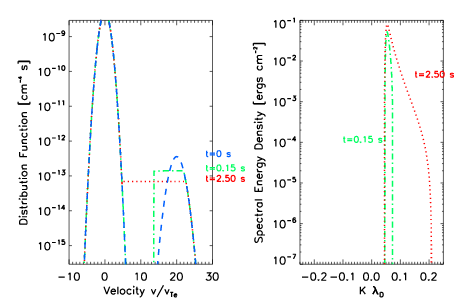
\includegraphics[width=0.75\columnwidth]{Images/L_wave_growth.png}
    \caption[Langmuir wave distriburtion function and spectral energy density.]{Left: Evolution of distribution function (normalised by the electron thermal velocity $v_{Te}=V_e$) in time. The diffusive term in \ref{eq:dfdt} causes the bump-on-tail Gaussian to turn into a plateau, thereby eliminating the instability caused by the positive velocity gradient. Right: The spectral energy density of generated Langmuir waves, x-axis normalised to the Debye length $\lambda_D=\sqrt{\frac{\epsilon_0 k_B T_e}{e^2 n_e}}$. As time passes the spectral range of Langmuir waves increases. Each panel shows successive times of t=0.15s (green, dot-dashed line) and t=2.50s (red, dotted line). \citep[Figure taken from][]{Reid2014}.} %(Figure taken from \citeauthor{Reid2014} \citeyear{Reid2014})}
    \label{fig:Lwavegrowth}
\end{figure}

\section{Wave-Wave Interaction}\label{Plasma Emission}
Wave-wave interaction concerns the processes by which three types of waves interact. These are: transverse (T) waves, Langmuir (L) waves and ion sound (S) waves, and have the following, respective dispersion relations,
$$ \omega=(\omega_p^2 +k^2c^2)^{\frac{1}{2}} $$
$$ \omega \cong \omega_p + \frac{3k^2V_e^2}{2 \omega_p}$$
$$ \omega = kv_s $$
where $V_e$ is the thermal velocity of electrons in the plasma, $v_s$ is the ion sound speed and $k$ is the wave vector. Only transverse waves with $\omega > \omega_p $ can escape and thus a plasma emission mechanism is a process that generates these transverse waves. 

As mentioned in Section \ref{characteristics}, Type III bursts have a harmonic structure associated with plasma emission at the plasma frequency and the second harmonic. Both of these transverse waves are formed in different three wave processes that will now be discussed.
In a plasma, due to scattering from other wave modes and ions in the plasma, a wave mode can be changed from one to the other. This is expressed in the equation 
$$ \sigma \rightleftarrows \sigma' + \sigma '' $$
where $\sigma$, $\sigma'$  and  $\sigma ''$ represent different wave modes. Conservation of energy and momentum state,
$$ \omega^{\sigma}(k)=\omega^{\sigma'}(k')+\omega^{\sigma''}(k'')$$
$$ k=k'+k''$$
where $ \omega^{\sigma}(k)$ is the frequency of a particular wave mode with the wave vector $k$. For Langmuir (L), ion sound (S) and transverse (T) wave modes the allowed processes are L+S$\rightarrow$L', L+S$\rightarrow$T,  T+S$\rightarrow$L,  T+S$\rightarrow$T' and  L+L'$\rightarrow$T. Of these L+S$\rightarrow$T,  L$\rightarrow$T+S are responsible for fundamental emission while harmonic emission is associated with the three wave process L+L'$\rightarrow$T.

Originally \cite{Ginzburg1958} considered fundamental emission to be due to Langmuir waves scattering off of thermal ions in the plasma. It is now commonly accepted that the biggest cause of fundamental emission is due to the three wave processes of a Langmuir wave coalescing with an ion sound wave generated by L$\rightarrow$L'+S or when a Langmuir wave decays into an ion sound wave and an electromagnetic transverse wave. The process L$\rightarrow$T+S can be visualised as in Figure \ref{fig:Femission}. In solar radio physics it is often assumed that $k_L \gg k_T$, knowing this and that the wave vectors must satisfy $\mathbf{k}_L \pm \mathbf{k}_s = \mathbf{k}_T$ ($+$ for L+S$\rightarrow$T , $-$ for L$\rightarrow$T+S) implies $\mathbf{k}_s \approx \mp \mathbf{k}_L$ 

\begin{figure}
\centering
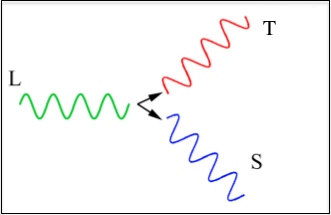
\includegraphics[width=0.5\columnwidth]{Images/Fundamental_emission_Lwaves.png}
\caption[A three wave process of fundamental plasma emission L$\rightarrow$T+S]{A three wave process of fundamental plasma emission L$\rightarrow$T+S. A Langmuir wave decaying into an ion sound wave and an electromagnetic transverse wave at the plasma frequency. (Figure adapted from Solar (interplanetary) Radio Bursts: the Generation of Radio Waves,	an oral presentation by David Malaspina at the Jean Louis Steinberg International Workshop on Solar, Heliospheric and Magnetospheric Radioastronomy, November 2017)}
\label{fig:Femission}
\end{figure}

Second harmonic emission occurs when two Langmuir waves coalesce in the process L+L'$\rightarrow$=T, shown in Figure \ref{fig:Hemission}. Conservation of momentum requires that $\mathbf{k}_L + \mathbf{k'}_L = \mathbf{k}_T$ and for second harmonic (H) generation, $k_T=k_H \approx \frac{\sqrt{3} \omega_p}{c}$. The phase speed $v_\phi$ of Langmuir waves is much less than $\frac{c}{\sqrt{3}}$ meaning that $k_L \gg k_T$ which results in $\mathbf{k}_L \approx -\mathbf{k'}_L$. This means that for a transverse wave at the second harmonic to be created, two Langmuir waves must coalesce almost exactly head on. These backward propagating Langmuir waves are generated: in the three wave processes of L+S$\rightarrow$L' and L$\rightarrow$L'+S; scattering off of thermal ions; and refraction at density inhomogeneities.
 \begin{figure}

     \centering
     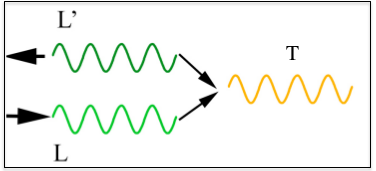
\includegraphics[width=0.5\columnwidth]{Images/Harmonic_emission_Lwaves.png}
     \caption[Three wave process of second harmonic plasma emission L+L' $\rightarrow$ T]{Three wave process of second harmonic plasma emission L+L' $\rightarrow$ T. A Langmuir wave (L) and a backwards propagating Langmuir wave (L') coalesce to form a transverse wave (T) at $2 \omega_p$. (Figure adapted from Solar (interplanetary) Radio Bursts: the Generation of Radio Waves,	an oral presentation by David Malaspina at the Jean Louis Steinberg International Workshop on Solar, Heliospheric and Magnetospheric Radioastronomy, November 2017)}
     \label{fig:Hemission}
 \end{figure}
 
\chapter{2017-10-15 Type III Burst}
\label{app:event}
The Type III burst which occurred at 13:21 UTC is shown in the composite radio spectra in Figure \ref{fig:comp_spec} and was not co-temporal with any other solar event.
EUV images of the Sun such as those taken in the 193{\AA} channel with AIA, Figure \ref{fig:AIA_GOES}a, show a number of bright active regions and a coronal hole which give indications of where to expect closed and open magnetic field lines.
Xray flux around the time of the Type III burst was measured by the Geostationary Operational Environmental Satellite (GOES, seen in Figure \ref{fig:AIA_GOES}b). It should be noted that there were a number of small C class solar flares before the radio burst however none were co-temporal. 
\newline
\begin{figure}[h]
    \centering
    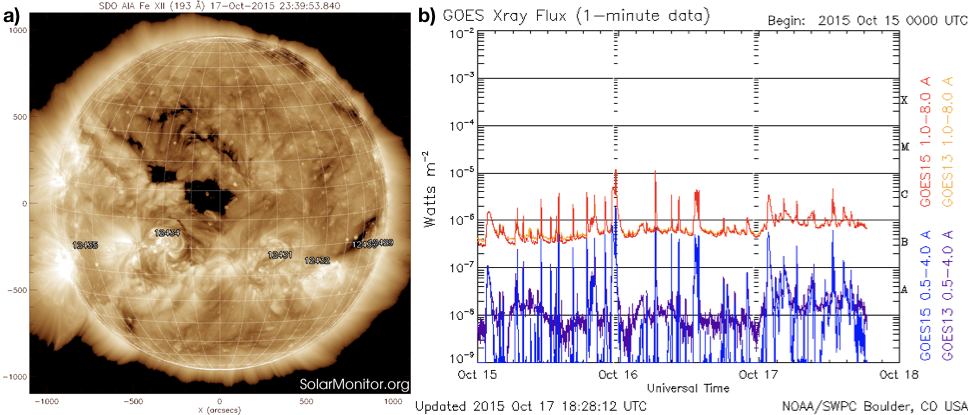
\includegraphics[width=0.75\columnwidth]{Images/aia_goes.png}
    \caption[193 {\AA} image of the Sun taken by AIA and Xray flux as measured by GOES on 2015-10-17]{a) 193 {\AA} image of the Sun taken by AIA on 2015-10-17 b) Xray flux as measured by GOES on 2015-10-17.}
    \label{fig:AIA_GOES}
\end{figure}

\begin{figure}
    \centering
    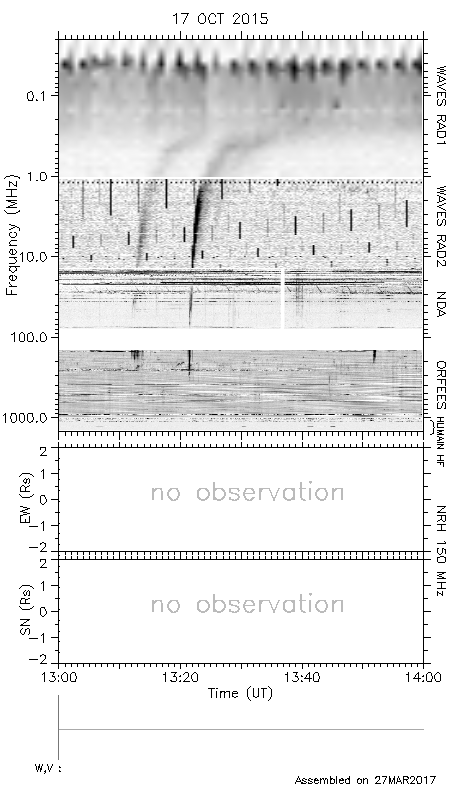
\includegraphics[width=0.75\columnwidth]{Images/Radio_composite.png}
    \caption[Composite of radio spectra from multiple ground and space based radio telescopes.]{Composite of radio spectra from multiple ground and space based radio telescopes. From top to bottom these include; WAVES RAD1, WAVES RAD2 (both on board the WIND space craft), the Nan\c{c}ay Decametric Array (NDA), ORFEES radio-spectrograph (Observations Radio pour Fedome et l’Etude des Eruptions Solaires) and the Nan\c{c}ay Radio Heliograph (NRH, no data). A Type III radio burst is seen as a dark streak after 13:20 in all 4 spectra.}
    \label{fig:comp_spec}
\end{figure}






% \begin{figure}
%     \centering
%     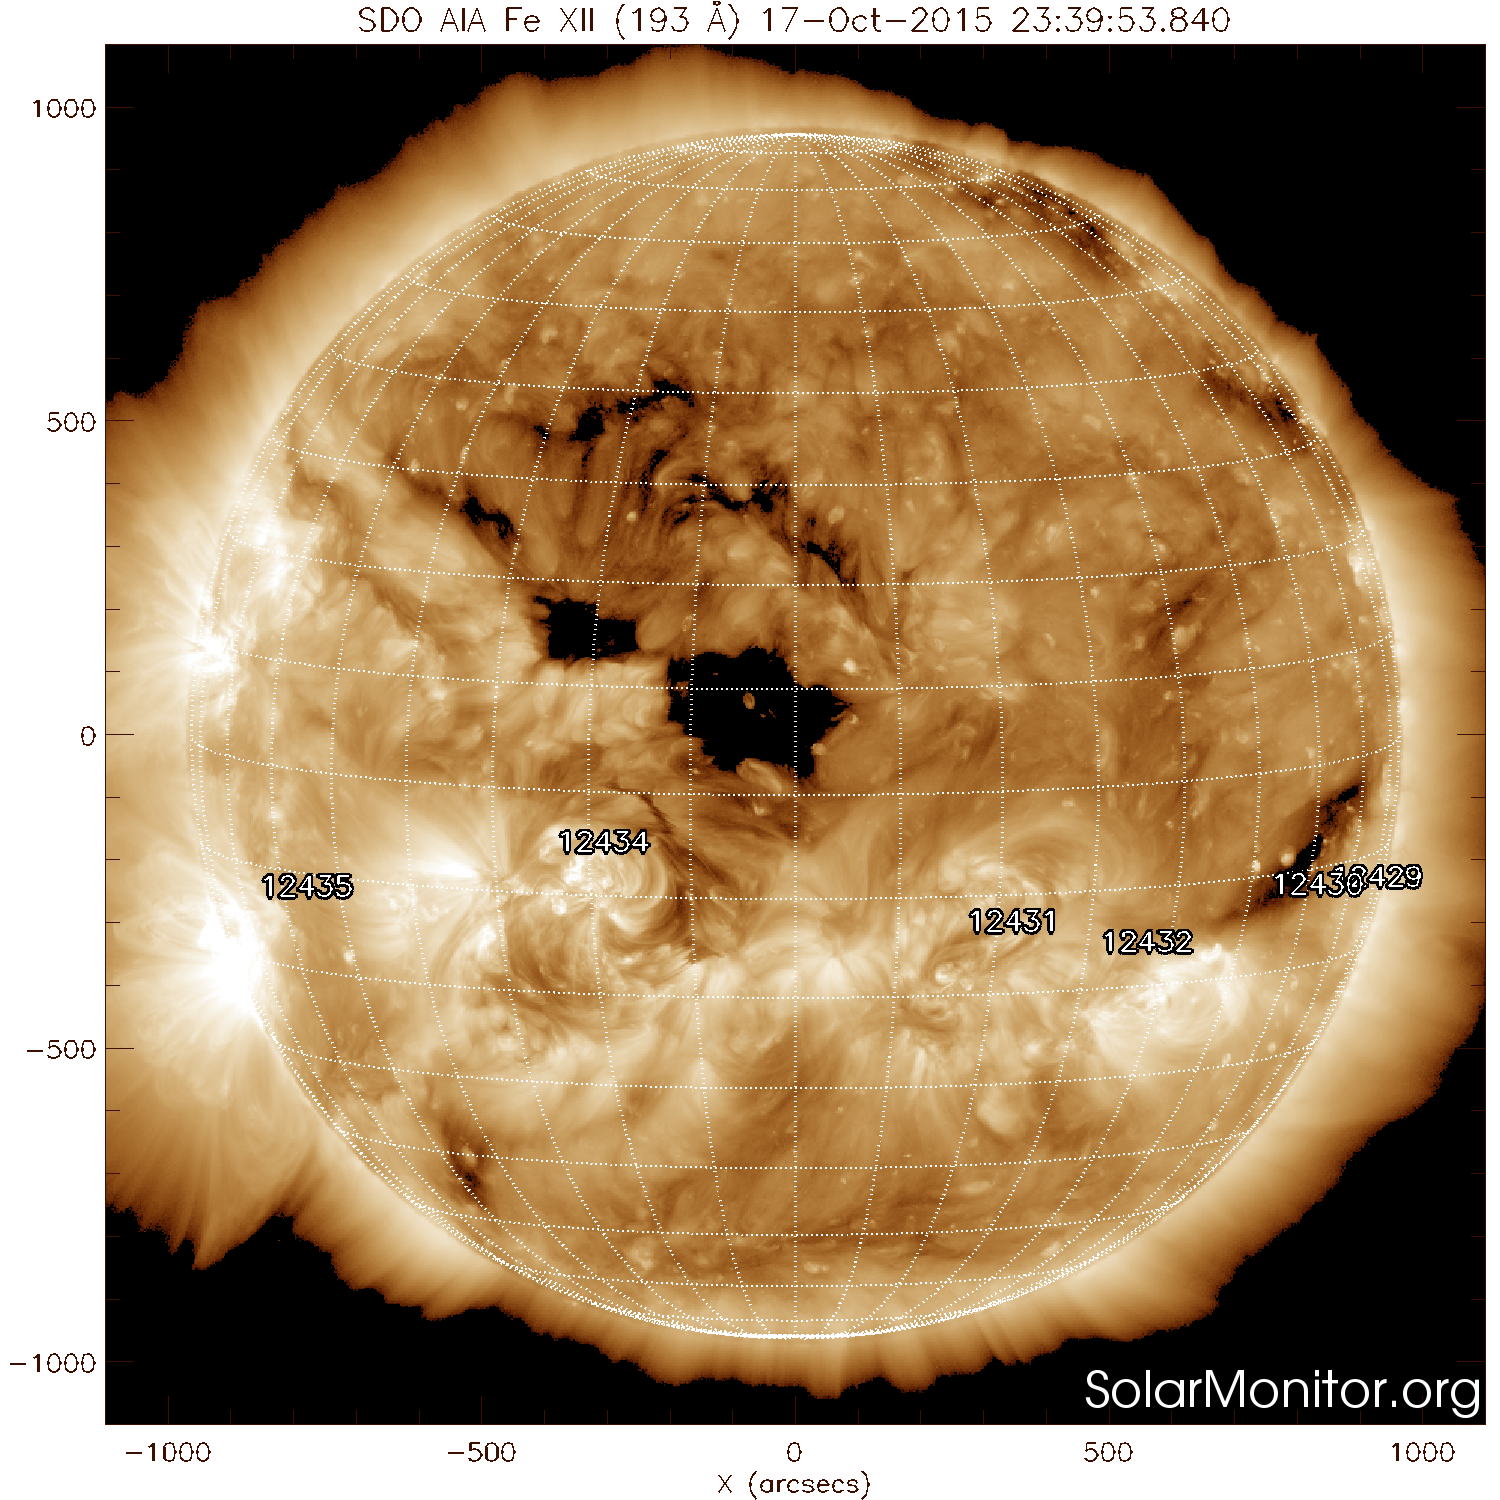
\includegraphics[width=0.75\columnwidth]{Images/aia_193.png}
%     \caption[193 {\AA} image of the Sun taken by AIA on 2015-10-17]{193 {\AA} image of the Sun taken by AIA on 2015-10-17}
%     \label{fig:aia193}
% \end{figure}

% A spectrum of the Sun was recorded using the LOFAR remote station RS509 from 2015-10-17 08:00 UTC to 2015-10-17 14:00 UTC. The Type III burst is observed in this spectrum approximately 19300s after the observation start as shown in Figure \ref{fig:LOFAR_spec}a. Figure \ref{fig:LOFAR_spec}b shows the burst over a shorter time scale thus allowing the variability in emission to be seen. It is immidiately obvious that the Type III burst shows striations, the implications of this will be discussed below.
% \begin{figure}
%     \centering
%     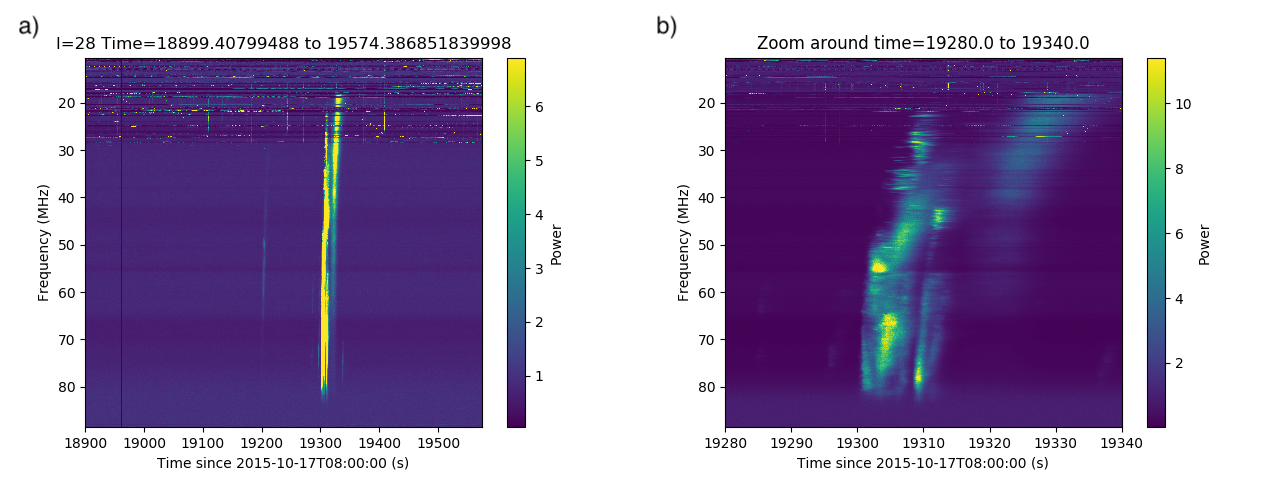
\includegraphics[width=\columnwidth]{Images/L401005_SAP000_B000_S0_P000_bf_d_spec_composite.png}
%     \caption[Type III radio burst observed with LOFAR station RS509]{a) Type III radio burst observed with LOFAR station RS509 in the north of the Netherlands. b) A zoom in of the Type III burst, a  plethora of temporal and frequency variation can be seen over the burst's duration.}
%     \label{fig:LOFAR_spec}
% \end{figure}


\end{document}

